\documentclass[11pt,a4paper]{article}
\usepackage[T1]{fontenc}
\usepackage{lmodern}
\usepackage{textcomp}
\usepackage{amsmath,amssymb,amsthm,mathtools}
\usepackage[textwidth=440pt,top=27mm,bottom=27mm]{geometry}
\usepackage{microtype}
\usepackage{xcolor}
\usepackage{tikz}
\usepackage{flafter,needspace}
\usepackage[colorlinks=true,linkcolor=blue!45!black,citecolor=blue!45!black,urlcolor=blue!45!black]{hyperref}
\hypersetup{pdftitle={A structural proof of the Karpelevic theorem},pdfauthor={Brecht Verbeken and Vincent Ginis}}
\newcommand{\R}{\mathbb R}
\newcommand{\C}{\mathbb C}
\newcommand{\Z}{\mathbb Z}
\DeclareMathOperator{\conv}{conv}
\DeclareMathOperator{\aff}{aff}
\DeclareMathOperator{\relint}{relint}
\DeclareMathOperator{\ext}{ext}
\DeclareMathOperator{\Arg}{Arg}
\newtheorem{theorem}{Theorem}[section]
\newtheorem{lemma}[theorem]{Lemma}
\newtheorem{proposition}[theorem]{Proposition}
\newtheorem{corollary}[theorem]{Corollary}
\theoremstyle{definition}
\newtheorem{definition}[theorem]{Definition}
\newtheorem{example}[theorem]{Example}
\theoremstyle{remark}
\newtheorem{remark}[theorem]{Remark}
\numberwithin{equation}{section}
\setlength{\emergencystretch}{1em}
\begin{document}
% BEGIN focused-frontmatter.tex
\title{A structural proof of the Karpelevi\v{c} theorem}
\author{Brecht Verbeken\textsuperscript{1,2} and Vincent Ginis\textsuperscript{1,2,3}}
\date{Research draft, 9 September 2026}
\maketitle
\begin{abstract}
We give a self-contained proof of the Karpelevi\v{c} theorem by reducing an extremal invariant polygon to a cyclic product with an exact real phase. A minimum branching count organizes the contacts, and face persistence makes a projective deformation applicable without separate tower-height cases. Convexity determines the sharp radius; explicit stochastic realizations and an independent Farey comparison identify the complete boundary. The resulting scalar equation also gives a uniform relative asymptotic for the radial deficit, including points arbitrarily close to Farey endpoints. It yields an $N^{-3}$ loss in badly approximable directions and a worst-direction loss of order $N^{-2}$ for optimal polygonal gauges.
\end{abstract}

\noindent\textit{Keywords.} Stochastic matrices; invariant polygons;
Karpelevi\v{c} theorem; Farey sequences; polyhedral Lyapunov functions.\par
\noindent\textit{2020 Mathematics Subject Classification.}
Primary 15A18, 15B51; Secondary 11J04, 52A10, 93D30.

\section{The boundary theorem}
Let $\Theta_n$ be the set of individual eigenvalues of real row-stochastic matrices of order $n$. Let $F_n$ list the reduced fractions in $[0,1]$ with denominator at most $n$, in increasing order, and put $F_n^+=F_n\cap[0,1/2]$. We prove the following form of the Karpelevi\v{c} theorem \cite{Karp,Ito}.

\begin{theorem}[Karpelevi\v{c}, in Ito form]\label{thm:karpelevic}
For $n\ge4$, consecutive fractions $f<g$ in $F_n^+$ determine one upper boundary arc of $\Theta_n$. Orient the pair so that the smaller denominator comes first: use $(p/q,r/s)=(f,g)$ and $\omega=z$ when the left denominator is smaller, and $(p/q,r/s)=(1-g,1-f)$ and $\omega=\bar z$ otherwise. Thus $q<s$ and $rq-ps=1$. With $m=\lfloor n/q\rfloor$, the arc is the branch of
\begin{equation}\label{eq:main-ito}
 \omega^s(\omega^q-\beta)^m=(1-\beta)^m\omega^{mq},
 \qquad 0\le\beta\le1,
\end{equation}
joining the corresponding roots of unity. More explicitly, on an interior ray put $\vartheta=\arg\omega\in(0,2\pi)$ and
\[
 A=q\vartheta-2\pi p,\qquad B=\frac{2\pi r-s\vartheta}{m}.
\]
Its boundary radius is the unique $\rho\in(0,1)$ solving
\[
 \rho^{s/m}\sin A+\rho^q\sin B=\sin(A+B).
\]
These arcs, in increasing argument, form the upper boundary. The lower boundary is their complex conjugate, and $\Theta_n$ consists of all radial segments from zero to the boundary.

The unit-circle points are exactly the roots of unity of orders at most $n$. The small orders are
\[
 \Theta_1=\{1\},\qquad \Theta_2=[-1,1],\qquad
 \Theta_3=\conv\{1,e^{2\pi i/3},e^{-2\pi i/3}\}\cup[-1,-1/2].
\]
The order-three terminal upper boundary is the vertical segment from $e^{2\pi i/3}$ to $-1/2$, followed by $[-1,-1/2]$.
\end{theorem}

\subsection*{The intermediate product}

The geometric part has a precise destination, stated fully in
Theorem~\ref{thm:product}. Take a nonreal radial extremum inside the
open unit disk, at its least matrix order $N\ge4$. For one choice of conjugate multiplier
$\omega=\rho e^{i\vartheta}$, a suitably chosen invariant polygon yields
Farey neighbors $p/q<\vartheta/(2\pi)<r/s$, with $q<s$, and coefficients
$0\le\beta_j<1$. With $m=\lfloor N/q\rfloor$ and $e=s-mq$, they satisfy
\[
 \omega^e\prod_{j=1}^{m}(\omega^q-\beta_j)
       =\prod_{j=1}^{m}(1-\beta_j),
 \qquad
 e\vartheta+\sum_{j=1}^{m}u_j=2\pi(r-mp).
\]
Here $u_j$ is the argument of the same factor $\omega^q-\beta_j$ in
$[A,M)$, where $A=q\vartheta-2\pi p$ and
$M=\Arg(\omega^q-1)\in(A,\pi)$. If $e<0$, the first identity is
understood for $\omega\ne0$, or after clearing the negative power.
The second identity is an equality of real numbers, not just a congruence.

The half-open contact convention fixes these arguments, and the tower
paths retain their total winding. Once both identities are available,
the phase fixes the mean argument and the modulus fixes a sum of convex
one-factor values. Equality of the coefficients then follows from the
sharp comparison. The geometry therefore needs to produce one such
optimized contact representation; it does not classify every invariant
polygon at the extremal eigenvalue.

\subsection*{Relation to earlier work}

Dmitriev and Dynkin obtained early restrictions on stochastic eigenvalues and determined the small orders \cite{DD}; Karpelevi\v{c} described the region in every order \cite{Karp}. \DJ okovi\'c later gave a simplification using cyclic polygons generated by powers of a complex number \cite{Djokovic}. Ito's polynomial formulation \cite{Ito} makes the boundary description especially concise. His argument establishes its equivalence with Karpelevi\v{c}'s theorem. A direct proof must instead explain why these polynomials describe the boundary, starting from the stochastic eigenvalue problem itself.

Realization, continuation, and outermostness are distinct parts of that task. Johnson and Paparella construct stochastic matrices realizing the roots of the relevant Ito polynomials \cite[Theorem~3.2]{JP}. Munger, Nickerson, and Paparella organize a direct proof around three assertions: realization, a continuous selection joining the appropriate roots of unity through a Farey interval, and extremality of that selection on its rays \cite[Proposition~1.2]{MNP}. Kirkland, Laffey, and \v{S}migoc give a scalar trigonometric characterization of the unique boundary point on a prescribed ray, taking the Karpelevi\v{c} boundary description as an input \cite[Theorems~1.1 and~1.2]{KirklandLaffeySmigoc}. In the present proof the product relation is derived from an arbitrary radial extremum. The convex comparison and an independent Farey refinement argument then identify its radius. The same scalar equation is recovered within the proof, before it is used for the later asymptotics.

The structure of realizing matrices has also been studied in greater detail than is needed for existence. Kirkland and \v{S}migoc classify realizations of the Type~0 and Type~I reduced Ito polynomials and the sparsest realizations of Types~II and~III \cite{KirklandSmigoc}. The subsequent preprints \cite{VGTypeII,VGTypeIII} treat the non-degenerate full-degree Type~II case and the Type~III realization conjecture over its stated nonzero parameter range. These classifications concern matrices attached to prescribed boundary polynomials. Theorem~\ref{thm:independent-realization} keeps the Johnson--Paparella graph and permits its return weights to vary independently. A cycle expansion computes the full characteristic polynomial. Appendix~\ref{app:matrix-family} records the graph's structural consequences and uses the convex comparison to identify the equal-weight tuple at the outer radius on the prescribed real phase. This last qualification is essential: the larger polynomial family also has roots on other phase branches.

The unrestricted region provides a reference point for structured stochastic families. Kirkland determined the non-Perron single-eigenvalue region of stochastic Leslie matrices in every order \cite{KirklandLeslie}. For matrices supported on a directed cycle and the diagonal, Ran and Teng formulated a four-dimensional conjecture \cite[Conjecture~20]{RanTeng}; the four-cycle region and its extension to every order are treated in \cite{VagenendeFourCycle,VGNCycle}. Work on monotone stochastic matrices determines the region through order three, provides realizations, and gives an all-order reduction \cite{VagenendeMonotone}. Star-convexity for stochastic eigenvalue regions and several subclasses is studied in \cite{VagenendeStar}. These are questions about the union of individual eigenvalues over a matrix family, which is different from prescribing the whole spectral list of one matrix.

Additional structural constraints also indicate where a further extension would require new arguments. The doubly stochastic single-eigenvalue problem belongs to the Perfect--Mirsky programme \cite{PerfectMirsky}. The proposed region is exact through order four \cite{LevickPereiraKribs}, but fails in order five \cite{HarlevJohnsonLim}. Doubly stochastic matrices, higher-order monotone matrices, and sparse support classes are therefore natural comparison problems for a theory based on phase-constrained products. The present paper proves no boundary classification for these additional families.

\Needspace{9\baselineskip}
\subsection*{Proof strategy and consequences}

The proof is self-contained apart from elementary linear algebra, the Perron--Frobenius theorem, and basic convexity and calculus. The segment comparison in Section~6 uses the one-variable fundamental theorem of calculus along a complex line segment; its application is to the polynomial $z^m$. Standard references for the background are Berman and Plemmons \cite{BermanPlemmons}, Schneider \cite{Schneider}, Coxeter \cite{Coxeter}, and Hardy and Wright \cite{HardyWright}. We prove the invariant-polygon correspondence, the deflation and projective statements, the return arithmetic, and the stochastic realization used below. No part of the Karpelevi\v{c} boundary theorem is used as an input.

The invariant-polygon correspondence and boundary-contact principle of Dmitriev and Dynkin \cite{DD}, also developed in Swift's account \cite{Swift}, turn the spectral question into one about a contracting rotation $T$. At a radial maximum of least order, every image vertex must meet the polygon boundary. Here this follows by removing a little stationary mass from a stochastic realization and normalizing its Perron eigenvector. We give the stationary-vector proof of this classical rank-one deflation principle \cite{Brauer,Goddard}.

The geometric reduction follows Karpelevi\v{c}'s architecture of vertex replacement, finite-rotation data, and a projective deformation forcing adjacent return \cite{Karp}. Here it is governed by the number of vertex images that lie inside sides. That count cannot increase under an intermediate invariant hull with the same number of vertices. Exchanging two stochastic factors moves these contacts while preserving the spectrum; minimizing their number before area places them in one interval. The remaining obstruction is a first return that skips over a base vertex. A general fact about invariant polytopes---the dimension of the smallest face containing an orbit point cannot decrease---supplies the exposing lines. An explicit positive-denominator chart makes the transfer through the convex chain a positive affine recursion in reciprocal coordinates. Its closing comparison moves one image vertex strictly inward while preserving every other incidence, contradicting boundary contact.

The deterministic paths can now be contracted to a cyclic product. A cyclic recurrence with side-dependent coefficients already occurs in Karpelevi\v{c}'s proof \cite[Theorem~VI and equation~(13)]{Karp}; he equalizes the coefficients geometrically before eliminating the vertices. We retain the unequal coefficients in the product together with their integer winding, since the product equation alone would not specify the boundary branch. After normalization, the factors lie on one affine line. The one-factor logarithmic convexity developed for the restricted $n$-cycle family \cite[Lemmas~4.2 and~5.2]{VGNCycle} then gives the sharp scalar upper bound and forces equality of the coefficients at the boundary. A cycle expansion on the Johnson--Paparella graph proves attainment. For the comparison between orders, one segment-integral identity handles both sides of a Farey mediant. This compares a least-order radial maximum with the candidate at the prescribed order.

The completed boundary theorem also solves an optimization problem for
polygonal gauges. For a rotation followed by multiplication by $\rho$,
the optimal gauge factor among polygons with at most $N$ vertices
is exactly $\rho/K_N(\theta)$. Section~\ref{sec:gauges} proves attainment
and the sharp worst-angle value. Section~\ref{sec:asymptotic} derives
the Farey asymptotic from the exact scalar equation, including relative
control arbitrarily close to either endpoint. This gives the different
vertex budgets for a fixed badly approximable direction and for a
guarantee uniform in direction.

Two refinements of the factor argument are collected after these
consequences. Appendix~\ref{app:comparisons} quantifies the Jensen gap
and treats unequal local exponents through a capped allocation of
angular deficits. Appendix~\ref{app:matrix-family} develops the
independent-parameter family already constructed in the main proof:
it records irreducibility, primitivity, sparsity, and endpoint matrices.
The convex comparison identifies the equal-parameter member that
attains the outer radius on the prescribed real phase.
These refinements are not prerequisites for the boundary proof.

This argument develops the geometric strategy and consequences of the
supplied manuscript \cite{VG}. The structural reductions and the
comparisons are proved here, so the paper can be read independently of
that manuscript.

% END focused-frontmatter.tex

% BEGIN focused-foundations.tex
\Needspace{8\baselineskip}
\section{Saturation and cyclic contacts}
For $n\ge1$, let $\Theta_n$ be the union of the spectra of all real row-stochastic matrices of order $n$. This set is compact, conjugation invariant, and contained in the closed unit disk: the stochastic matrices form a compact set, their operator norm on $\ell^\infty$ is one, and the equation $\det(\lambda I-A)=0$ is closed. The inclusions $\Theta_n\subseteq\Theta_{n+1}$ follow by adjoining an identity block.

The invariant-polygon correspondence of Dmitriev and Dynkin \cite[\S\S1--2]{DD}, presented in English by Swift \cite{Swift}, is
\begin{equation}\label{eq:polygon-criterion}
 \lambda\in\Theta_n\quad\Longleftrightarrow\quad
 \begin{gathered}
 \lambda P\subseteq P\text{ for a non-singleton polytope }P\subset\C\\
 \text{with at most }n\text{ vertices}\quad(n\ge2).
 \end{gathered}
\end{equation}
Indeed, from $Av=\lambda v$ take $P=\conv\{v_1,\ldots,v_n\}$. If it is a singleton then $\lambda=1$, for which any segment works. Conversely, expressing each $\lambda v_i$ as a convex combination of the vertices gives a stochastic eigenpair, which can be padded with an identity block.
For nonreal $\lambda$, such a polytope is a polygon: a segment would give a real invariant line. For nonreal $\lambda$ with $0<|\lambda|\le1$, one has $0\in\operatorname{int}P$. Iteration puts $0$ in $P$ when $|\lambda|<1$; when $|\lambda|=1$, the averages of a nonzero rotational orbit tend to zero and do the same. In either case, a supporting half-plane through $0$ would then contain an entire rotational orbit of a nonzero vector. A finite such orbit sums to zero and an infinite one is dense in the circle, so neither fits in that half-plane.

The sets $\Theta_n$, $n\ge2$, are star-shaped about zero. If $Av=\lambda v$, $\lambda\ne1$, choose a stationary probability row vector $\pi^T$. Then $\pi^Tv=0$ and
\[
 [tA+(1-t)\mathbf1\pi^T]v=t\lambda v\qquad(0\le t\le1).
\]
For $\lambda=1$, the matrix with rows $(1,0)$ and $(1-t,t)$ realizes $t$. Write $R_n(t)$ for the maximum radius on the ray of argument $t$.

For the geometric reduction, fix a nonreal multiplier $\zeta=\rho e^{i\theta_\zeta}$, $0<\rho<1$, satisfying
\begin{equation}\label{eq:extremal}
 \begin{gathered}
 \min\{|\ext P|:\zeta P\subseteq P,\ \operatorname{int}P\ne\varnothing\}=N,\\
 \text{for every }t>1,\quad t\zeta\text{ has no invariant polygon}\\
 \text{with at most }N\text{ vertices}.
 \end{gathered}
\end{equation}
Write $Tz=\zeta z$. These hypotheses hold at the first order of occurrence of any nonreal radial maximum inside the unit disk. A real planar map with nonreal eigenvalues is real-linearly conjugate to multiplication by either eigenvalue, so this entails no loss of generality.

\paragraph{Notation and orientation.}
The upper-half-plane point in the boundary theorem is $z$.
The geometric argument may choose its conjugate: $\zeta$ denotes the
multiplier after arranging the half-open contacts, and
$\theta_\zeta\in(0,2\pi)$ denotes its argument. The product theorem
then chooses $\omega\in\{\zeta,\overline\zeta\}$ so that the smaller
Farey denominator comes first; its argument is $\vartheta$.
Every conjugation replaces an argument by $2\pi$ minus that argument
and reverses the vertex list. It reflects an ordered Farey pair
$(f,g)$ to $(1-g,1-f)$. Section~5 returns to the upper ray
$\theta=\arg z\in(0,\pi)$ and explicitly makes this final choice of
$\omega$.

The integer notation follows the successive reductions:
\begin{center}
\begin{tabular}{@{}p{0.23\linewidth}p{0.71\linewidth}@{}}
$N,\kappa,\delta$ & Least matrix order, cyclic contact shift, and
 $\delta=\gcd(N,\kappa)$.\\[3pt]
$\varphi$ & Number of interior contacts after they form one interval.\\[3pt]
$\nu,q,h,\Delta$ & In the arithmetic suspension, the number of bases,
 short return time, excess return time, and return displacement.
 For the contact towers $\nu=\varphi$; the product construction reapplies the lemma
 with a possibly larger set of bases.\\[3pt]
$\ell$ & Length of the convex chain in the projective lemma.\\[3pt]
$q,s,m,e$ & In the product, the ordered Farey denominators,
 the factor count $m=\lfloor N/q\rfloor$, and $e=s-mq$.
 These data are specified anew in each return case.
\end{tabular}
\end{center}

\subsection{Perron deflation forces boundary contact}
A rank-one eigenvalue shift, due to Brauer \cite{Brauer} and developed further by Goddard \cite{Goddard}, gives the saturation needed throughout the proof. The contact conclusions go back to Dmitriev and Dynkin \cite[\S\S1--2]{DD}; the deflation argument below proves them in the hereditary form needed for later replacements. Subtracting a multiple of the stationary row leaves the other eigendirections unchanged while decreasing the Perron root. A positive diagonal normalization then moves those eigenvalues radially outward. A positive row provides enough room to make this subtraction without changing the support.

\begin{lemma}[Positive Perron deflation]\label{lem:perron-deflation}
Let $A$ be irreducible stochastic with stationary probability vector $\pi^T$.
If $u\ge0$, $B=A-u\pi^T$ is nonnegative and irreducible, and $r=1-\pi^Tu\in(0,1)$, then a positive diagonal similarity makes $B/r$ stochastic.
Its non-Perron eigenvalues are those of $A$ divided by $r$, including algebraic multiplicities.
Such a deflation exists whenever $A$ has a positive row.
\end{lemma}
\begin{proof}
The identity $\pi^TB=r\pi^T$, with $\pi>0$, identifies $r$ as the Perron root of $B$.
For $Bh=rh$, $h>0$, put $D=\operatorname{diag}(h)$; then $r^{-1}D^{-1}BD\mathbf1=\mathbf1$.
On the invariant hyperplane $\ker\pi^T$, $B$ agrees with $A$, whereas its quotient eigenvalue is $r$.
This proves the spectral assertion, and an eigenvector $v$ becomes $D^{-1}v$.
If row $i$ is positive, take $u=\varepsilon e_i$ with
$0<\varepsilon<\min_j(a_{ij}/\pi_j)\le1$; $B$ retains the support of $A$ and $r\in(0,1)$.
\end{proof}

\begin{theorem}[Hereditary saturation]\label{thm:saturation}
Under \eqref{eq:extremal}, every invariant polygon with at most $N$ vertices has exactly $N$ vertices; every image vertex belongs to its boundary; and every side meets its image.
\end{theorem}
\begin{proof}
Let $v_1,\ldots,v_N$ be the vertices of such a polygon and choose a stochastic realization $Av=\zeta v$ by barycentric coordinates.
Every such $A$ is irreducible: a proper nonempty closed row set would restrict this equation to a smaller stochastic realization, whose eigenvector is nonzero because every polygon vertex is nonzero.
That contradicts minimal order.

If $\zeta v_i$ were interior, its barycentric coordinates could all be chosen positive, making row $i$ positive.
To see this, first assign a small equal weight to every vertex; the remaining point is still in the polygon.
Lemma~\ref{lem:perron-deflation} would then realize $\zeta/r$ stochastically at order $N$, with $r<1$, contradicting radial maximality and \eqref{eq:polygon-criterion}.
Thus every image vertex is on the boundary.

The polar polygon $P^\circ=\{a:\langle a,x\rangle\le1\text{ for all }x\in P\}$ has one vertex for each side of $P$.
It is invariant under the adjoint map, since $\langle T^*a,x\rangle=\langle a,Tx\rangle\le1$; that map satisfies the same hypotheses by reflection.
Apply the vertex-contact conclusion to it.
For a polar vertex $a$, the boundary point $T^*a$ satisfies $\langle T^*a,x\rangle=1$ for some $x\in P$.
Hence $\langle a,Tx\rangle=1$, so the side of $P$ exposed by $a$ meets $TP$.
\end{proof}

We use the following elementary face rule: if a positive convex combination of points of a polytope lies on its boundary, every point used lies in one common proper face.
A supporting functional proves this by equality in its upper bound.
For a polygon, positive support at a saturated contact therefore consists of at most two adjacent vertices.

\subsection{Branching monotonicity}
The number of vertices is fixed by minimal order. A second integer makes clipping monotone. For an injective linear map $T$ and a $T$-invariant polytope $P$ with vertex set $V$, define
\[
 d_T(P)=|\{v\in V:Tv\in V\}|,\qquad
 b_T(P)=|V|-d_T(P).
\]
The first counts deterministic contacts; the second counts images that are not vertices. In a saturated planar realization, these are precisely the images inside edges.

\begin{theorem}[Monotonicity under intermediate hulls]\label{thm:branching}
In any dimension, suppose
\[
 TP\subseteq Q\subseteq P,\qquad
 |\ext Q|=|\ext P|,\qquad
 \ext Q\subseteq\ext P\cup T\ext P.
\]
Then $Q$ is invariant and $b_T(Q)\le b_T(P)$.
\end{theorem}
\begin{proof}
Put $W=\ext Q$, $R=V\setminus W$, $A=W\setminus V$, and $E=\{v\in V:Tv\in V\}$. An extreme point of $P$ lying in $Q$ remains extreme in $Q$. Hence $R\cap TV=\varnothing$. Every old deterministic source in $E\setminus R$ therefore remains deterministic. Since $A\subset TV$, injectivity makes $S=T^{-1}A$ a subset of $V$ of size $|A|=|R|$, disjoint from $E$. The retained sources $S\setminus R$ are new deterministic sources for $Q$, disjoint from the old ones. Consequently
\[
 d_T(Q)\ge |E|-|E\cap R|+|R|-|S\cap R|
 \ge |E|-|E\cap R|+|R|-|R\setminus E|=|E|.
\]
Finally $TQ\subseteq TP\subseteq Q$.
\end{proof}

Normalize the invariant $N$-gons in \eqref{eq:extremal} by
\[
 \max_{x\in P}|x|=1.
\]
The normalized class is compact. Indeed, from any sequence choose a convergent subsequence of the $N$-tuples of vertices in the closed unit disk. Their limiting convex hull remains invariant, contains zero, and has radius one. The last two properties exclude a point. Nonreality of $\zeta$ excludes a segment, and minimal order excludes a polygon with fewer than $N$ vertices. Thus all $N$ limiting points are distinct vertices.

In these vertex coordinates, an equality $Tv_i=v_j$ can appear in a limit but cannot disappear. The count $d_T$ is therefore upper semicontinuous, and $b_T$ is lower semicontinuous. Its minimum is attained on a compact set; continuity of area then gives an area minimizer within that set. Choose such a polygon $P$ throughout this section: it minimizes $(b_T(P),\operatorname{area}(P))$ lexicographically in the normalized class, meaning first branching, then area. Scaling changes neither count, so its branching count is minimal among all invariant $N$-gons, with or without the normalization.

These two choices have different uses. For an intermediate hull with $N$ vertices drawn from $\ext P\cup T\ext P$, Theorem~\ref{thm:branching} preserves minimum branching. If that hull also retains a radius-one vertex, it is still normalized; a proper inclusion would then contradict the area choice. Later interchanges will retain minimum branching even when they do not retain the area choice.

\subsection{The cyclic contact representation}
Write $[a,b]_{\partial P}$ for the boundary arc from $a$ to $b$ in the positive direction, with the indicated endpoints included or excluded. The half-open sides $(v_{i-1},v_i]$ partition $\partial P$: each vertex belongs to the side ending there. We must choose an orientation in which these sides receive exactly one image vertex each. Boundary contact alone does not yet specify which side receives a contact at a vertex.

List the vertices $y_j$ of $TP$ in cyclic order. Saturation puts them on $\partial P$, in the same order, and ensures that every side of $P$ meets $TP$. For the image edge $[y_j,y_{j+1}]$, intersect $P$ with the closed half-plane bounded by its line and containing $TP$; call the intersection $Q_j$. Let
\[
 k_j=|\ext P\cap[y_j,y_{j+1}]_{\partial P}|.
\]
If the cut is proper, its line meets the interior of $P$. The two boundary intersections are therefore exactly $y_j,y_{j+1}$, and the discarded boundary is the positive open arc between them. The cut removes the old vertices on that open arc and can add only its two endpoints. Counting both endpoints in $k_j$ gives
\[
 TP\subseteq Q_j\subsetneq P,\qquad
 |\ext Q_j|\le N+2-k_j.
\]
The intermediate hull is invariant, so minimal order forces $k_j\le2$. When $k_j=2$, it has exactly $N$ vertices and all its new vertices lie in $T\ext P$. Theorem~\ref{thm:branching} therefore puts it in the same minimum-branching class.

Fix a vertex $v_*$ of $P$ with $|v_*|=1$. Every $y_j$ has radius at most $\rho<1$, so $v_*$ lies on exactly one of the disjoint open arcs $(y_j,y_{j+1})_{\partial P}$. A proper cut with $k_j=2$ must discard $v_*$: otherwise $Q_j$ would remain normalized and branch-minimal, but have strictly smaller area than $P$. Hence at most one proper cut has $k_j=2$. If $Q_j=P$, the image-edge line supports $P$, and the arc lies on one side; its positive half-open part contains at most one old vertex.

The closed-arc bound controls the cuts. To determine endpoint assignments, set
\[
 r_j=|\ext P\cap(y_j,y_{j+1}]_{\partial P}|,
 \qquad \varepsilon_j=\mathbf1_{\{y_j\in\ext P\}}.
\]
These half-open arcs partition the old vertex set. Consequently
\[
 \sum_j r_j=N,\qquad k_j=r_j+\varepsilon_j,\qquad 0\le r_j\le2,
\]
and at most one $r_j$ equals two. Either every $r_j=1$, or there are unique indices $s,t$ with
\[
 r_s=2,\qquad r_t=0,\qquad r_j=1\quad(j\notin\{s,t\}).
\]
Consider the latter case. Since $k_s\le2$, necessarily $\varepsilon_s=0$. Also $\varepsilon_{s+1}=1$. Otherwise the two old vertices counted by $r_s$ would both lie strictly between $y_s$ and $y_{s+1}$. They are consecutive vertices of $P$, and their joining side contains no image vertex. It could not meet $TP$: a supporting functional attaining its maximum on $TP$ attains it at an image vertex. This contradicts side contact. Thus $s$ is a transition from zero to one in the cyclic sequence $(\varepsilon_j)$.

A transition from one to zero can occur only at $t$. Indeed, suppose $\varepsilon_j=1$ and $\varepsilon_{j+1}=0$ with $j\ne t$. Then $j\ne s$, so $r_j=1$ and $k_j=2$. This cut must be proper. If its line supported $P$, the arc would start at the old vertex $y_j$ and end at the nonvertex $y_{j+1}$ on that side, before the next old vertex; it would then have $r_j=0$. The proper cut at $j$ would therefore be a second one with $k_j=2$, a contradiction.

A cyclic binary sequence has equally many transitions in the two directions. The upward transition at $s$ and the only possible downward transition at $t$ must therefore be its only transitions. Switching which endpoint belongs to an arc gives
\[
 |\ext P\cap[y_j,y_{j+1})_{\partial P}|
 =r_j+\varepsilon_j-\varepsilon_{j+1}=1
 \quad\text{for every }j.
\]
Thus one of the two half-open conventions interlaces the vertex lists exactly. If each $[y_j,y_{j+1})_{\partial P}$ contains the old vertex $u_j$, then $y_j\in(u_{j-1},u_j]$. If instead each $(y_j,y_{j+1}]_{\partial P}$ contains $u_j$, then $y_{j+1}\in[u_j,u_{j+1})$. In this second case replace $P$ by $\overline P$ and $\zeta$ by $\overline\zeta$, and list the reflected vertices in positive cyclic order. This converts the assignment into sides open at their initial endpoint. Conjugation preserves the extremality hypotheses \eqref{eq:extremal}, the branching count, normalization, and area. Retain the notation $P,\zeta$ for the resulting polygon and multiplier.

Multiplication by $\zeta$ preserves cyclic order. The resulting bijection from source vertices to half-open target sides is therefore a translation of cyclic index sets. For a uniquely determined $1\le\kappa\le N$,
\begin{equation}\label{eq:contacts}
 c_i=\zeta v_{i-\kappa}
 =\beta_i v_{i-1}+\alpha_i v_i\in(v_{i-1},v_i],
 \qquad \alpha_i=1-\beta_i>0,
\end{equation}
with indices modulo $N$. If $\kappa=N$, every contact is interior, and conjugating with reversed vertex order gives the same representation with $\kappa=1$ and interchanged coefficients. We henceforth arrange $1\le\kappa<N$.

Choose vertex arguments $\Phi_i$ increasing with $i$, extended by $\Phi_{i+N}=\Phi_i+2\pi$. Since $0$ is interior, each gap $\gamma_i=\Phi_i-\Phi_{i-1}$ lies in $(0,\pi)$. Polar argument increases along each side, so, for the representative $0<\theta_\zeta<2\pi$ of $\arg\zeta$,
\begin{equation}\label{eq:lift}
 \Phi_{i-1}<\Phi_{i-\kappa}+\theta_\zeta\le\Phi_i,
 \qquad \frac{\kappa-1}{N}<\frac{\theta_\zeta}{2\pi}<\frac\kappa N.
\end{equation}
There is no hidden multiple of $2\pi$ in the first inequality, because both its interval after subtracting $\Phi_{i-\kappa}$ and $\theta_\zeta$ lie between zero and $2\pi$. Summing gives the second assertion; equality on the right would make every contact deterministic and force a nonzero vertex to be fixed by a positive power of $\zeta$, contrary to $|\zeta|<1$.

\subsection{The local operation and the global normal form}
The local replacement exchanges two stochastic factors. If $A=HS$ with
$H,S$ stochastic and $S$ invertible, then
\[
 A'=SH=SAS^{-1}
\]
is stochastic with the same spectrum, and an eigenvector $v$ becomes
$Sv$. We choose $S$ to move one polygon vertex into its preceding side.

Let $C$ act on lists by $(Cv)_r=v_{r+1}$, and let $B(\beta)$ have row $i$ equal to $\beta_i e_{i-1}^T+\alpha_i e_i^T$. Then \eqref{eq:contacts} is the stochastic eigenpair
\[
 A=C^\kappa B(\beta),\qquad Av=\zeta v.
\]
For the deterministic idempotent $E_i$ that sends coordinate $i$ to $i-1$ and fixes the others, put $S_i(t)=(1-t)I+tE_i$.

The coefficients are most transparent as nonnegative weights
$w_i=-\log\alpha_i$. The update below transports one such weight
along the cyclic shift and adds it to the weight at its destination:
\[
 w_i'=0,\qquad w_{i+\kappa}'=w_i+w_{i+\kappa}.
\]
The factor swap supplies stochasticity and the eigenpair; saturation
will ensure that the modified row still uses only one polygon side.

\begin{lemma}[Positive interchange]\label{lem:interchange}
If $\beta_i=t>0$ and $\beta_{i+1}=0$, replacing $v_i$ by $c_i$ gives another saturated invariant $N$-gon with the same cyclic shift. Its coefficients satisfy
\begin{equation}\label{eq:coalescence}
 \alpha_i'=1,\qquad \alpha_{i+\kappa}'=\alpha_i\alpha_{i+\kappa},
 \qquad \alpha_j'=\alpha_j\quad(j\notin\{i,i+\kappa\}).
\end{equation}
The corresponding stochastic matrices are similar.
\end{lemma}
\begin{proof}
Write $\widehat B$ for $B$ with its $i$th row changed to $e_i^T$, and set
$S=S_i(t)$, $H=C^\kappa\widehat B$.
Since the only other row that could use column $i$ is row $i+1$, whose coefficient there is zero,
\[
 B=\widehat B S,\qquad A=HS,\qquad A'=SH=SAS^{-1}.
\]
Here $S^{-1}=(I-tE_i)/(1-t)$, and both $H$ and $S$ are stochastic.
Hence $v'=Sv$ satisfies $A'v'=\zeta v'$ and its convex hull is invariant. It has at most $N$ vertices, hence exactly $N$ by minimal order. Its displayed points remain in the original cyclic order: only $v_i$ moves into its preceding side. Saturation applies.

Put $j=i+\kappa$, so $j\ne i$. Moving the elementary factor through $C^\kappa$ gives $A'=C^\kappa S_j(t)\widehat B$. Only row $j$ of $\widehat B$ is changed, to
\[
 t\widehat\beta_{j-1}e_{j-2}^T
 +\bigl(t\widehat\alpha_{j-1}+(1-t)\beta_j\bigr)e_{j-1}^T
 +(1-t)\alpha_j e_j^T.
\]
The coefficients at $j-1$ and $j$ are positive because $0<t<1$ and every $\widehat\alpha$ is positive. This row represents a boundary contact of the new polygon. The face rule forces all its positive support into one side, and the vertices $v'_{j-1},v'_j$ already determine that side. It follows that $\widehat\beta_{j-1}=0$: otherwise the third vertex $v'_{j-2}$ would belong to it. These three vertices are distinct because $N\ge3$. This argument also covers $j-1=i$, when the hatted coefficient is already zero.

The coefficient at $j$ is $(1-t)\alpha_j=\alpha_i\alpha_j$, while all other rows agree with $\widehat B$. This proves \eqref{eq:coalescence}. The coefficient at the terminal vertex of each side remains positive, so the same shift and half-open assignment are retained.
\end{proof}

The support $I=\{i:w_i>0\}=\{i:\beta_i>0\}$ therefore changes to
$(I\setminus\{i\})\cup\{i+\kappa\}$. Minimum branching will forbid
a collision of two positive weights; the area choice will place their
support in one interval.

\begin{proposition}[Branch-minimal normal form]\label{prop:interval}
The chosen polygon has, after cyclic relabelling,
\[
 I=\{1,\ldots,\varphi\},\qquad \varphi\ge\delta:=\gcd(N,\kappa).
\]
If $\varphi<N$, it is the deficit of a record of the rotation by $\kappa$: for some $h>0$,
\begin{equation}\label{eq:record}
 [h\kappa]_N=N-\varphi,
 \qquad [t\kappa]_N<N-\varphi\quad(0\le t<h).
\end{equation}
For $\varphi=N$, use the time-zero record.
\end{proposition}
\begin{proof}
Every $\kappa$-orbit meets $I$; otherwise all contacts along that orbit would be endpoints, and their identities would give $v=\zeta^{N/\delta}v$. Suppose $I$ is proper. At the last index $i$ of any cyclic component, $\beta_i>0$ and $\beta_{i+1}=0$, so Lemma~\ref{lem:interchange} applies. Moving the extreme vertex $v_i$ into its preceding side gives a proper subpolygon. The support formula shows that its branching count cannot increase, and global minimality prevents it from decreasing.

Apply this operation separately at each component end of the chosen polygon $P$. The replacement point $c_i=\zeta v_{i-\kappa}$ has radius at most $\rho<1$. If any radius-one vertex other than $v_i$ remained, the new polygon would still be normalized and branch-minimal, with strictly smaller area. Therefore $v_i$ must be the unique radius-one vertex. Two different component ends cannot both have this property. Hence $I$ is one interval; since it meets every residue class modulo $\delta$, its size is at least $\delta$.

For the record assertion assume $\varphi<N$ and temporarily label the interval $F\cup\{0\}$, where $F=\{N-\varphi+1,\ldots,N-1\}$. Let $a_t=[t\kappa]_N$, and let $h$ be its first positive entrance into $\{N-\varphi,\ldots,N-1\}$. Such an entrance exists because this set of $\varphi\ge\delta$ consecutive residues contains a multiple of $\delta$, and the orbit of zero consists of all those multiples.

Before that entrance, follow the branching contact initially at zero. In the state $F\cup\{a_t\}$ one has $a_t<N-\varphi$, so $a_t+1\notin F\cup\{a_t\}$ and the interchange is allowed at $a_t$. It moves this contact to $a_{t+1}$ and leaves $F$ in place. If $a_{t+1}\in F$, the two branching contacts coalesce and the branching count drops by one, contrary to its global minimum. Otherwise the count is unchanged, and the new state is $F\cup\{a_{t+1}\}$. These later polygons need not minimize area; minimum branching is preserved, since a rescaling would put any one of them back in the normalized class without changing its count.

At the first entrance, every target except $N-\varphi$ lies in $F$. The forbidden collision therefore gives $a_h=N-\varphi$, with all earlier residues smaller. Relabelling the original interval back to $\{1,\ldots,\varphi\}$ leaves these residue displacements unchanged.
\end{proof}

% END focused-foundations.tex

% BEGIN focused-returns.tex
\Needspace{12\baselineskip}
\section{Return geometry}
\subsection{Arithmetic suspension}\label{sec:return-arithmetic}
An endpoint contact gives the exact identity $\zeta v_i=v_{i+\kappa}$.
Starting from an interior-contact index, these identities can be followed
until the next such index is reached. We call the intervening list of
indices a tower. Its height records how many applications of $\zeta$
have been contracted, while the unreduced index advance records how
many turns have been made. Both quantities will enter the product
equation. We first determine the towers by arithmetic alone.

The record basis reformulates Karpelevi\v{c}'s analysis of Euclidean
remainders \cite[\S3, Lemma~2 and Theorems~III--IV]{Karp}.
Slater studies related gap and return phenomena for rotations
\cite{Slater}; Hardy and Wright give the Farey background
\cite[Chapter~III]{HardyWright}. The finite suspension and its endpoint
conventions are proved explicitly here.

Fix $1\le\kappa<N$, $\delta=\gcd(N,\kappa)$, and define $L(a,b)=a\kappa-bN$. A record time $h$ is a strict record for $[h\kappa]_N$, with deficit $\nu=N-[h\kappa]_N$. At time zero take $V=(0,1)$ and $\nu=N$; otherwise take $V=(h,\lceil h\kappa/N\rceil)$. The last record has deficit $\delta$.

\begin{lemma}[Record basis]\label{lem:record-basis}
For consecutive records $V=(h,b)$ and $V'$, whose deficits are $\nu>\nu'$, put $U=V'-V=(q,p)$ and $\Delta=\nu-\nu'$. Then
\begin{equation}\label{eq:record-basis}
 \det(U,V)=1,\quad L(U)=\Delta,\quad L(V)=-\nu,
 \quad q\nu+h\Delta=N,\quad \gcd(\Delta,\nu)=\delta.
\end{equation}
In particular $q>0$ and $0<\Delta<\nu$.
\end{lemma}
\begin{proof}
The attainable residues are the multiples of $\delta$, so the last deficit is $\delta$. Every record vector is primitive: if $V=gW$, $g>1$, then the earlier time of $W$ would have the smaller positive deficit $\nu/g$. Also
\[
 -\det(V,V')=\frac{h'\nu-h\nu'}{N}>0.
\]
If this integer is $D>1$, complete the primitive vector $V$ to an integer basis $(V,W_0)$ by B\'ezout, choosing its orientation so that $V'=aV+DW_0$. Primitivity of $V'$ gives $\gcd(a,D)=1$. Thus
\[
 W=\left(\lceil a/D\rceil-a/D\right)V+D^{-1}V'
   =\lceil a/D\rceil V+W_0
\]
is a nonzero integer point $\alpha V+\beta V'$ with $0<\alpha,\beta<1$. Replacing $W$ by $V+V'-W$ if necessary gives $\alpha+\beta\le1$. Its time is strictly between zero and $h'$, while
\[
 0<-L(W)=\alpha\nu+\beta\nu'<\nu.
\]
It would therefore improve the first record before the second one, a contradiction. Thus $\det(U,V)=1$. The remaining identities follow by applying $L$ to the basis and expanding its determinant. In particular $L(\Z^2)=\delta\Z=\Delta\Z+\nu\Z$.
\end{proof}

The identity $q\nu+h\Delta=N$ suggests $\nu-\Delta$ towers of height
$q$ and $\Delta$ towers of height $q+h$: their heights sum to $N$.
The congruences determine where their tops return. To prove that these
lists really partition all indices, it remains to exclude repetitions.
The following argument does this using the cycles of the base
permutation. It requires only the displayed integer relations, so it
can also be used later with a different choice of bases.

\Needspace{19\baselineskip}
\begin{lemma}[Arithmetic suspension]\label{lem:suspension}
Suppose positive integers $\nu,\Delta,q$ and $h\ge0$ satisfy $1\le\Delta\le\nu$, $\nu\le N$,
\[
 \begin{gathered}
 q\kappa\equiv\Delta\pmod N,\qquad h\kappa\equiv-\nu\pmod N,\\
 q\nu+h\Delta=N,\qquad \gcd(\Delta,\nu)=\gcd(\kappa,N)=\delta.
 \end{gathered}
\]
On the bases $J=\{1,\ldots,\nu\}$ define
\[
 H_j=q+h\mathbf1_{\{j>\nu-\Delta\}},\qquad
 \sigma(j)=j+\Delta\pmod\nu
\]
with values in $J$. Then
\[
 \pi(t,j)=[j+t\kappa]_N,\qquad j\in J,\ 0\le t<H_j,
\]
is a bijection onto $\Z/N\Z$. The first return of addition by $\kappa$ to $J$ has time $H_j$ and destination $\sigma(j)$.
\end{lemma}
\begin{proof}
Regard the pairs $(t,j)$ as abstract states before identifying them
with residues. Advance from $(t,j)$ to $(t+1,j)$ inside a tower, and
from $(H_j-1,j)$ to $(0,\sigma(j))$ at its top. Under $\pi$, an internal
step is addition by $\kappa$. A top step has the same property: for a
short tower $q\kappa\equiv\Delta$, and for a long tower
$(q+h)\kappa\equiv\Delta-\nu$, exactly accounting for the wrap in
$\sigma(j)$.

The base permutation has $\delta$ cycles, one for each residue class
modulo $\delta$. Each has $\nu/\delta$ bases and $\Delta/\delta$ long
bases, since the long block has length $\Delta$ and both lengths are
divisible by $\delta$. Each resulting suspension cycle therefore has
\[
 q\nu/\delta+h\Delta/\delta=N/\delta
\]
states. Addition by $\kappa$ also has period $N/\delta$, so the images
of those states are one entire $\kappa$-orbit, without repetition.
Different base cycles map to different residue classes modulo $\delta$.
This proves bijectivity. In particular, no internal state can represent
an element of $J$, since that residue is already represented by its
base state $(0,j)$. The displayed heights are therefore the first
return times, including when $\nu=\Delta=1$.
\end{proof}

Apply the record lemma at the deficit $\varphi$ supplied by Proposition~\ref{prop:interval}, provided $\varphi>\delta$. The time-zero record has next record $(1,1)$, so it is included. We obtain
\begin{equation}\label{eq:tower-data}
 q\kappa-pN=\Delta,\qquad h\kappa-bN=-\varphi,
 \qquad q\varphi+h\Delta=N,\qquad
 1\le\Delta<\varphi,\quad\gcd(\Delta,\varphi)=\delta.
\end{equation}
Every internal destination in this suspension lies outside
$I=\{1,\ldots,\varphi\}$, so its contact equation is an endpoint
identity. At the top, the destination belongs to $I$: the image is
the contact on the side ending at $v_{\sigma(j)}$, rather than that
vertex itself. Thus the arithmetic first returns give the geometric
identities
\begin{equation}\label{eq:towers}
 \zeta^t v_j=v_{\pi(t,j)}\ (0\le t<H_j),\qquad
 \zeta^{H_j}v_j=c_{\sigma(j)},\qquad
 \zeta^h v_\varphi=v_0,\quad \zeta^qv_0=c_\Delta.
\end{equation}
Here the closing state is $\pi(h,\varphi)=0$, with $h<H_\varphi=q+h$.

For example, take $N=8$, $\kappa=3$, and the record deficit
$\varphi=2$. The record occurs at $h=2$, and the next record gives
$q=3$ and $\Delta=1$. The two towers are
\[
\begin{array}{c|c|c|c}
\text{base }j&H_j&\text{indices before return}&\sigma(j)\\ \hline
1&3&1,4,7&2\\
2&5&2,5,0,3,6&1
\end{array}
\]
Each residue occurs once. For a contact representation with these
data, the corresponding closing equations are
$\zeta^3v_1=c_2$ and $\zeta^5v_2=c_1$; the second tower also contains
$\zeta^2v_2=v_0$. We continue this example after
Theorem~\ref{thm:product}, where the paths give both a polynomial and
its real phase. The arithmetic construction alone does not assert
the existence of an invariant polygon with prescribed contact data.

Reducing all indices modulo $N$ would lose the winding needed to
select the boundary branch. We therefore retain the lifted vertex
arguments $\Phi_{i+N}=\Phi_i+2\pi$ from \eqref{eq:lift}. Along an
endpoint path of length $t$, starting at index $a$,
\begin{equation}\label{eq:path-lift}
 \Phi_a+t\theta_\zeta=\Phi_{a+t\kappa}.
\end{equation}
If only its last contact is interior, the right-hand side is replaced by the open interval $(\Phi_{a+t\kappa-1},\Phi_{a+t\kappa})$. The index $a+t\kappa$ is an integer, not merely a residue. Composition adds path lengths and index advances. Consequently contracting deterministic paths preserves the integer winding as well as the complex eigenvalue equation.

% END focused-returns.tex

% BEGIN focused-holonomy.tex
% Focused replacement: boundary persistence, positive holonomy, no skipping.
% Dependencies: eq:contacts, eq:tower-data, eq:towers, thm:saturation.
\subsection{Face persistence and projective transfer}

Karpelevi\v{c}'s proof uses a projective deformation to force adjacent
return \cite{Karp}. We retain that geometric purpose, using face
persistence to supply its exposing lines. The projective facts needed
below are derived in coordinates; Coxeter \cite{Coxeter} gives the
standard background on perspectivities and projectivities.

For an injective affine map with $F(P)\subseteq P$, let $G_P(x)$ be
the minimal face of $P$ containing $x$.  Then
\[
 F(G_P(x))\subseteq G_P(Fx),\qquad
 \dim G_P(x)\le\dim G_P(Fx).
\]
Indeed, $x\in\relint G_P(x)$, so every supporting functional at $Fx$
pulls back to a functional constant on $G_P(x)$.  This proves the
inclusion, and injectivity gives the dimension inequality.  In particular,
a nonvertex can never become a vertex.  In the plane this says that an
image can pass from a side into the interior, but cannot pass from a side
interior to a vertex.  The half-open contact assignment gives a more
precise conclusion when an entire side remains on the boundary: it
identifies the endpoint that must remain a vertex.

\begin{lemma}[Boundary persistence and one-sided exposure]
\label{lem:boundary-persistence}
Assume the half-open contact assignment \eqref{eq:contacts} for the
invertible map $F$, and write $E_i=[v_{i-1},v_i]$.
If $r\ge1$ is an integer and $F^rE_i\subseteq\partial P$, then
\[
 F^t v_{i-1}=v_{i-1+t\kappa}\qquad(0\le t\le r).
\]
Consequently, if $F^rv_i$ is in a side interior and $v_{i-1}$ has a
nonvertex image by time $r$, the inverse image of that side's line
exposes $v_i$.
\end{lemma}
\begin{proof}
Invertibility and $F(P)\subseteq P$ imply
$F(\operatorname{int}P)\subseteq\operatorname{int}P$.  Thus no point of
$FE_i$ can be interior: its subsequent image under $F^{r-1}$ is on the
boundary.  The nondegenerate boundary segment $FE_i$ must lie in one
side.  Its endpoints, however, have the adjacent half-open assignments
\[
 Fv_{i-1}\in(v_{i+\kappa-2},v_{i+\kappa-1}],\qquad
 Fv_i\in(v_{i+\kappa-1},v_{i+\kappa}].
\]
The second endpoint is beyond their common vertex, so the first endpoint
must equal that vertex.  Consequently
\[
 Fv_{i-1}=v_{i+\kappa-1},\qquad
 \relint(FE_i)\subseteq\relint E_{i+\kappa}.
\]

To repeat this argument, we need the whole next side, not just the
subsegment $FE_i$.  Choose $y\in\relint(FE_i)$.  It is a strict convex
combination of the endpoints of $E_{i+\kappa}$, while $F^{r-1}y$ lies
on the boundary.  A supporting functional there is maximal on both
images of those endpoints, because it is maximal on their strict convex
combination.  Hence $F^{r-1}E_{i+\kappa}\subseteq\partial P$.
Induction on $r$ now proves the asserted endpoint identities.

The pulled-back line supports $P$ at $v_i$.  If it also contained
$v_{i+1}$, the first assertion applied to $E_{i+1}$ would make
$F^rv_i$ a vertex.  If it contained $v_{i-1}$, the same assertion
applied to $E_i$ would make $F^rv_{i-1}$ a vertex, contrary to
persistence of nonvertices.  It therefore exposes $v_i$.
\end{proof}

We next isolate the geometric deformation that will be applied to the
exposing lines supplied by this lemma.  Exposure provides the lines along
which vertices may move; we still need a choice of motion that opens a
contact inward.  Its construction is local near
the original polygon, but the sign of the deformation is determined by
evaluating a projectivity at one remote point.  Completed lines allow
that evaluation even if an intermediate projection goes to infinity in
the original affine chart.

These projective operations can be read as linear algebra in homogeneous
coordinates: an affine point $(x,y)$ represents the
one-dimensional subspace spanned by $(x,y,1)$ in $\R^3$, and a completed
line is represented by a two-dimensional subspace.
Projection from a centre $c$ onto the line $\eta^TX=0$ is induced by
\[
 X\longmapsto\left(I-\frac{c\eta^T}{\eta^Tc}\right)X.
\]
If the centre is on neither line, this is an isomorphism between their
two-dimensional subspaces, hence a fractional-linear map of line coordinates.
An invertible $3\times3$ matrix changes the projective chart. Where its
affine denominator has constant sign, it preserves segments and their interiors.

\Needspace{20\baselineskip}
\begin{lemma}[Strict holonomy of a convex chain]\label{lem:chain-holonomy}
Let $X_0,\ldots,X_{\ell+1}$, with $\ell\ge2$, be distinct consecutive vertices
of a convex polygon, in either boundary orientation, whose indicated sides
do not exhaust its boundary.  Choose
\[
 C_i\in\relint[X_{i-1},X_i]\quad(2\le i\le \ell+1),
 \qquad P\cap L_i=\{X_i\}\quad(2\le i\le \ell),
\]
where each $L_i$ is a line.  Put $\Lambda_1=\aff(X_0,X_1)$ and
$K=\aff(C_\ell,C_{\ell+1})$.  Projection successively through $C_i$ onto $L_i$,
then through $X_{\ell+1}$ onto $K$, defines a projectivity $\Pi$ between
the completed lines satisfying
\begin{equation}\label{eq:strict-holonomy}
 \Pi(X_1)=C_{\ell+1},\qquad
 \Pi(X_0)\in\relint[C_{\ell+1},C_\ell].
\end{equation}
Suppose $S:\overline\Lambda_1\to\overline K$ is any projectivity with
$S(X_1)=C_{\ell+1}$ and $S(X_0)=C_\ell$.  For small real $t$ define
\[
 Y(t)=(1-t)C_{\ell+1}+tC_\ell,\qquad X_1(t)=S^{-1}(Y(t)),
 \qquad X_i(t)=L_i\cap\aff(X_{i-1}(t),C_i).
\]
There are arbitrarily small nonzero $t$ for which $Y(t)$ lies strictly
on the inward side of $\aff(X_\ell(t),X_{\ell+1})$.  The inward defect opens
to first order, or, if its first derivative vanishes, strictly to second
order.
\end{lemma}

\begin{figure}[htbp]
\centering
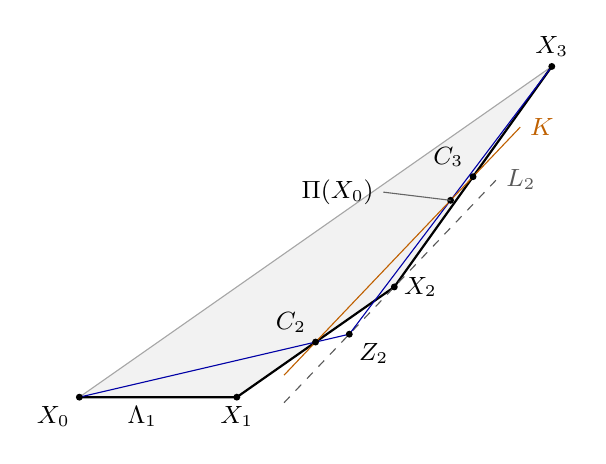
\begin{tikzpicture}[x=2cm,y=1.4cm, font=\small]
 \coordinate (X0) at (0,0);
 \coordinate (X1) at (1,0);
 \coordinate (X2) at (2,1);
 \coordinate (X3) at (3,3);
 \coordinate (C2) at (1.5,.5);
 \coordinate (C3) at (2.5,2);
 \coordinate (Z2) at ({12/7},{4/7});
 \coordinate (W) at ({33/14},{25/14});
 \fill[black!5] (X0)--(X1)--(X2)--(X3)--cycle;
 \draw[black!35] (X3)--(X0);
 \draw[thick] (X0)--(X1)--(X2)--(X3);
 \draw[dashed,black!65] (1.3,-.05)--(2.65,1.975)
   node[right] {$L_2$};
 \draw[blue!65!black] (X0)--(Z2)--(X3);
 \draw[orange!75!black] (1.3,.2)--(2.8,2.45)
   node[right] {$K$};
 \foreach \p in {X0,X1,X2,X3,C2,C3,Z2,W}
   \fill (\p) circle[radius=1.25pt];
 \node[below left] at (X0) {$X_0$};
 \node[below] at (X1) {$X_1$};
 \node[right] at (X2) {$X_2$};
 \node[above] at (X3) {$X_3$};
 \node[above left] at (C2) {$C_2$};
 \node[above left] at (C3) {$C_3$};
 \node[below right] at (Z2) {$Z_2$};
 \draw[black!60] (W)--(1.93,1.86);
 \node[left] at (1.93,1.86) {$\Pi(X_0)$};
 \node[below] at (.4,0) {$\Lambda_1$};
\end{tikzpicture}
\caption{The remote construction for a convex chain with $\ell=2$.
Projection from $C_2$ sends $X_0$ to $Z_2$; projection from $X_3$
then meets $K$ between $C_2$ and $C_3$.  Starting instead at $X_1$
gives $X_2$ and then $C_3$.}
\end{figure}

\begin{proof}
Every projection has its centre on neither source nor target line.  This
follows from exposure of the vertices and noncollinearity of adjacent sides;
for the final projection, $X_{\ell+1}\notin K$ because $C_\ell,C_{\ell+1}$ lie
in the interiors of different adjacent sides.  Thus all maps are
projectivities.  Their intersections are transverse at the original
configuration, so the displayed affine motion is finite and continuous
near zero.

Starting at $X_1$, each projection gives the next vertex $X_i$, and
the last projection gives $C_{\ell+1}$.  To locate $\Pi(X_0)$, we choose
a chart in which all slopes have a useful order.

Choose affine functions $\eta_0,\eta_1\ge0$ on $P$ that vanish there
only at $X_0,X_{\ell+1}$, respectively.  For example, at each endpoint
add inward defining functions of its two incident sides.  Their sum
$\eta=\eta_0+\eta_1$ is strictly positive on $P$, because the endpoints
are distinct.  The functions $\eta_0,\eta$ are independent, as their
values at the two endpoints show.  Choose an affine function $\psi$
completing them to a basis of the affine functions on the plane.  Then
\[
 \Phi(x)=\left(\frac{\eta_0(x)}{\eta(x)},
                  \frac{\psi(x)}{\eta(x)}\right)
\]
is an invertible projective change of chart, finite throughout $P$.
Moreover,
\[
 \Phi((1-s)x+sy)=
 \frac{(1-s)\eta(x)\Phi(x)+s\eta(y)\Phi(y)}
 {(1-s)\eta(x)+s\eta(y)}\qquad(0\le s\le1).
\]
The positive weights show directly that convexity, segments, and side
interiors are preserved.

The first coordinate has unique minimum zero at $X_0$ and unique maximum
one at $X_{\ell+1}$.  Each vertical slice of the polygon is an interval,
so its two boundary chains between these endpoints are graphs.  There
are no vertical sides: a vertical supporting line would give a horizontal
extremum, and both extrema are single vertices.  Reflect the second
coordinate if necessary to make the selected chain the lower graph.
The internal exposing lines are nonvertical for the same reason.
Consecutive genuine vertices give strictly increasing side slopes, and
exposure puts the slope of $L_i$ strictly between those of its two
incident sides.
Thus
\[
 X_i=(t_i,f_i),\quad t_0<\cdots<t_{\ell+1},\qquad
 d_1<\cdots<d_{\ell+1},\quad d_i<s_i<d_{i+1},
\]
where $d_i$ is the slope of its $i$th side and $s_i$ that of $L_i$.
Set $s_1=d_1$ and $h_i=t_i-t_{i-1}>0$.  Write the contacts and seek the
successive remote projections in the form
\[
 C_i=X_i-\gamma_i h_i(1,d_i),\quad0<\gamma_i<1,
 \qquad Z_i=X_i-r_i(1,s_i).
\]
The starting point $Z_1=X_0$ gives $r_1=h_1$.  At each step the required
collinearity is that of the vectors
\[
 \begin{split}
 C_i-Z_{i-1}&=(1-\gamma_i)h_i(1,d_i)+r_{i-1}(1,s_{i-1}),\\
 Z_i-C_i&=\gamma_i h_i(1,d_i)-r_i(1,s_i).
 \end{split}
\]
Their determinant is zero.  In reciprocal coordinates $x_i=1/r_i$,
expanding this determinant gives the affine transfer rule
\begin{equation}\label{eq:positive-transfer}
 x_i=\frac{(1-\gamma_i)(s_i-d_i)}{\gamma_i(d_i-s_{i-1})}x_{i-1}
       +\frac{s_i-s_{i-1}}{\gamma_i h_i(d_i-s_{i-1})}.
\end{equation}
Both its slope and its intercept are strictly positive, since
$s_{i-1}<d_i<s_i$.  Starting with $x_1=1/h_1>0$, it therefore gives
finite positive $x_i$.  The points defined by $r_i=1/x_i$ satisfy the
collinearity equations, so they are the unique projective intersections.
This proves their finiteness without assuming it in advance.
The positive intercept also gives the strict bounds
\[
 0<r_i<\gamma_i h_i\frac{d_i-s_{i-1}}{s_i-s_{i-1}}
          <\gamma_i h_i\qquad(2\le i\le\ell).
\]

For the final projection put $r=r_\ell$, $g=\gamma_{\ell}h_{\ell}$,
$H=h_{\ell+1}$, $d=d_\ell$, $s=s_\ell$, and $D=d_{\ell+1}$.  The signed line
functional $G(W)=\det(X_{\ell+1}-Z_\ell,W-Z_\ell)$ satisfies
\[
 \begin{split}
 G(C_\ell)&=H(g-r)(D-s)+g(H+r)(s-d)>0,\\
 G(C_{\ell+1})&=-\gamma_{\ell+1}Hr(D-s)<0.
 \end{split}
\]
The opposite signs place the final intersection strictly between the
two contacts, proving \eqref{eq:strict-holonomy}.

Return now to the original affine chart, where the deformation in the
statement is defined.  Use $z(t)=(1-t)C_{\ell+1}+tC_\ell$ as affine
coordinate on $K$.  The map
$\Pi\circ S^{-1}$ becomes
\[
 u(t)=\frac{at}{1+bt},\qquad a\ne0,\qquad u(0)=0,\quad0<u(1)<1.
\]
Consequently
\begin{equation}\label{eq:holonomy-defect}
 t-u(t)=\frac{(1-a)t+bt^2}{1+bt}.
\end{equation}
If $a\ne1$, choose the sign of $t$ so that $(1-a)t>0$.  If $a=1$,
then $0<u(1)<1$ forces $b>0$, and either sufficiently small nonzero
sign works.  The final moving line intersects $K$ at $z(u(t))$.
At zero, increasing the coordinate toward $C_\ell$ enters its inward
half-plane: $C_\ell$ is strictly inward from the final side.  More
explicitly, choose a continuous signed affine functional for the moving
line, positive on its inward side.  Its value at $z(t)$ is
$\Gamma(t)(t-u(t))$, with $\Gamma(0)>0$.  The positive factor persists
near zero, so \eqref{eq:holonomy-defect} proves both the inward motion
and its first- or second-order opening.  The calculation at the remote
parameter $1$ determines the sign of this local motion; it does not
require the affine construction to remain finite throughout $[0,1]$.
\end{proof}

The local sign is now settled, including the case of a vanishing first
variation.  To use it in an invariant polygon, we must also propagate the
motion along all vertex orbits and preserve every other terminal contact.
The next proof separates these global constraints by their side indices.

\begin{theorem}[No skipping in a saturated contact network]
\label{thm:no-skipping}
Assume hereditary saturation as in Theorem~\ref{thm:saturation},
$N\ge4$, and the return data \eqref{eq:tower-data}--\eqref{eq:towers}
for the exact interval of interior contacts
$B=\{1,\ldots,\varphi\}$, with $\varphi>\gcd(N,\kappa)$.
Then $\Delta=1$.
\end{theorem}
\begin{proof}
Write $F$ for multiplication by the chosen multiplier, and recall
\[
 \sigma(j)=1+[j+\Delta-1]_\varphi,\qquad
 H_j=q+h\mathbf1_{j>\varphi-\Delta},\qquad
 F^{H_j}v_j=c_{\sigma(j)},\quad F^hv_\varphi=v_0.
\]
The first nonvertex image of base $v_j$ occurs at time $H_j$; all
earlier tower steps are vertex identities.  For $j\ge2$, its predecessor
$v_{j-1}$ has already acquired a nonvertex image by that time, since
$H_{j-1}\le H_j$.  Lemma~\ref{lem:boundary-persistence} therefore gives
\[
 \mathcal L_j:=F^{-H_j}\aff E_{\sigma(j)}
 \quad\hbox{exposes }v_j\qquad(2\le j\le\varphi).
\]
This is also why the possible jump from height $q$ to height $q+h$
causes no difficulty: a nonvertex image remains a nonvertex throughout
the additional steps.

Suppose $\Delta>1$.  We shall deform the polygon while preserving
invariance and making one image vertex interior, contradicting saturation.
Choose the shorter of the two contact chains joining the seed to its
target, with orientation recorded by $\varepsilon$:
\[
 (\varepsilon,\ell,X_i,a)=
 \begin{cases}
 (1,\Delta,v_i,q),&2\Delta\le\varphi+1,\\
 (-1,\varphi-\Delta+1,v_{\varphi-i},q+h),&2\Delta>\varphi+1,
 \end{cases}
 \qquad 0\le i\le \ell+1.
\]
Here $2\le \ell\le(\varphi+1)/2$.  If $\varphi<N$, then $\ell+1\le\varphi<N$;
if $\varphi=N\ge4$, then $\ell+1\le(N+3)/2<N$.  Thus the chain is proper.
The endpoints are unmoved bases except possibly $X_0=v_0$, which is
fixed by the unmoved base $v_\varphi$ through $v_0=F^hv_\varphi$.
Take $L_i=\mathcal L_j$ when $X_i=v_j$, $2\le i\le \ell$; the indices lie
in $\{2,\ldots,\varphi\}$, so all these lines expose their vertices.
Let $C_i$ be the contact on $[X_{i-1},X_i]$.  In the two orientations,
\[
 (C_\ell,C_{\ell+1})=(c_\Delta,c_{\Delta+1})
 \quad\hbox{or}\quad(c_\Delta,c_{\Delta-1}),
\]
and the tower identities give $F^aX_0=C_\ell$, $F^aX_1=C_{\ell+1}$.

To extend the chain motion to the polygon, we must control both the
vertex identities inside towers and the side contacts at their ends.
Only sides $E_i$ with $i\in B$ carry terminal contacts.  Their endpoints
are bases, except $v_0=F^hv_\varphi$, which stays fixed.
Let $b$ be the index of $X_1$, $M$ the indices of $X_1,\ldots,X_\ell$,
$k_*:=\sigma(b)$ the final side index, and $J$ the internal side indices.
Reading each side by its ending vertex, in $\Z/\varphi\Z$ one has
\begin{equation}\label{eq:network-disjointness}
 \sigma(M)=\{k_*+\varepsilon t:0\le t<\ell\},\qquad
 J=\{k_*-\varepsilon r:1\le r<\ell\}.
\end{equation}
These arcs are disjoint, since an intersection would require
$\varphi\mid(t+r)$ with $1\le t+r\le2\ell-2<\varphi$.
Also $\sigma(b)=k_*$ and no other moving source targets that side.
Thus a changing internal side has a fixed terminal source, while every
moving source except the seed has a fixed target line.  Figure~\ref{fig:global-motion}
shows this separation together with the tower extension used below.

\begin{figure}[htbp]
\centering
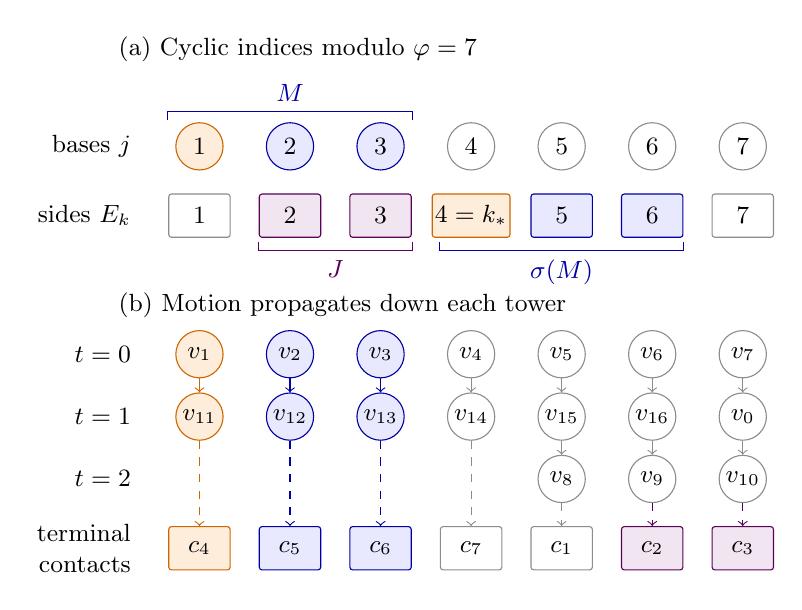
\begin{tikzpicture}[x=1.15cm,y=.88cm,font=\small,
 vertex/.style={circle,draw=black!45,fill=white,minimum size=6mm,inner sep=1pt},
 moving/.style={vertex,draw=blue!65!black,fill=blue!9},
 seed/.style={vertex,draw=orange!80!black,fill=orange!14},
 side/.style={draw=black!45,fill=white,rounded corners=1pt,
              minimum width=7.8mm,minimum height=5.5mm,inner sep=1pt},
 internal/.style={side,draw=violet!70!black,fill=violet!10},
 target/.style={side,draw=blue!65!black,fill=blue!9},
 exceptional/.style={side,draw=orange!80!black,fill=orange!14}]
 \node[anchor=west] at (0,7.55) {(a) Cyclic indices modulo $\varphi=7$};
 \node[anchor=east] at (.35,6.15) {bases $j$};
 \node[seed] at (1,6.15) {$1$};
 \foreach \j in {2,3} \node[moving] at (\j,6.15) {$\j$};
 \foreach \j in {4,5,6,7} \node[vertex] at (\j,6.15) {$\j$};
 \draw[blue!65!black] (.65,6.53)--(.65,6.65)--(3.35,6.65)--(3.35,6.53);
 \node[blue!65!black,above] at (2,6.65) {$M$};
 \node[anchor=east] at (.35,5.15) {sides $E_k$};
 \foreach \k in {1,7} \node[side] at (\k,5.15) {$\k$};
 \foreach \k in {2,3} \node[internal] at (\k,5.15) {$\k$};
 \node[exceptional] at (4,5.15) {$4=k_*$};
 \foreach \k in {5,6} \node[target] at (\k,5.15) {$\k$};
 \draw[violet!70!black] (1.65,4.77)--(1.65,4.65)--(3.35,4.65)--(3.35,4.77);
 \node[violet!70!black,below] at (2.5,4.65) {$J$};
 \draw[blue!65!black] (3.65,4.77)--(3.65,4.65)--(6.35,4.65)--(6.35,4.77);
 \node[blue!65!black,below] at (5,4.65) {$\sigma(M)$};
 \node[anchor=west] at (0,3.85) {(b) Motion propagates down each tower};
 \node[anchor=east] at (.35,3.15) {$t=0$};
 \node[anchor=east] at (.35,2.25) {$t=1$};
 \node[anchor=east] at (.35,1.35) {$t=2$};
 \node[seed] (B1) at (1,3.15) {$v_1$};
 \node[seed] (T1) at (1,2.25) {$v_{11}$};
 \foreach \j/\k in {2/12,3/13} {
   \node[moving] (B\j) at (\j,3.15) {$v_{\j}$};
   \node[moving] (T\j) at (\j,2.25) {$v_{\k}$};
 }
 \foreach \j/\k in {4/14,5/15,6/16,7/0} {
   \node[vertex] (B\j) at (\j,3.15) {$v_{\j}$};
   \node[vertex] (T\j) at (\j,2.25) {$v_{\k}$};
 }
 \foreach \j/\k in {5/8,6/9,7/10}
   \node[vertex] (U\j) at (\j,1.35) {$v_{\k}$};
 \draw[->,orange!80!black] (B1)--(T1);
 \foreach \j in {2,3} \draw[->,blue!65!black] (B\j)--(T\j);
 \foreach \j in {4,5,6,7} \draw[->,black!45] (B\j)--(T\j);
 \foreach \j in {5,6,7} \draw[->,black!45] (T\j)--(U\j);
 \node[exceptional] (C1) at (1,.35) {$c_4$};
 \foreach \j/\k in {2/5,3/6} \node[target] (C\j) at (\j,.35) {$c_{\k}$};
 \foreach \j/\k in {4/7,5/1} \node[side] (C\j) at (\j,.35) {$c_{\k}$};
 \foreach \j/\k in {6/2,7/3} \node[internal] (C\j) at (\j,.35) {$c_{\k}$};
 \draw[->,dashed,orange!80!black] (T1)--(C1);
 \foreach \j in {2,3} \draw[->,dashed,blue!65!black] (T\j)--(C\j);
 \draw[->,dashed,black!45] (T4)--(C4);
 \draw[->,dashed,black!45] (U5)--(C5);
 \foreach \j in {6,7} \draw[->,dashed,violet!70!black] (U\j)--(C\j);
 \node[anchor=east,align=right] at (.35,.35) {terminal\\contacts};
\end{tikzpicture}
\caption{The arithmetic schema $(N,\kappa,\varphi,\Delta,q,h)=(17,10,7,3,2,1)$,
with $\ell=3$ and $\sigma(j)=1+[j+2]_7$.
The moving bases are $M=\{1,2,3\}$; the internal chain sides
$J=\{2,3\}$ are disjoint from their targets $\sigma(M)=\{4,5,6\}$.
Solid arrows are exact vertex images under $F$; dashed arrows are the
terminal side contacts before deformation.  Coloured towers move by
\eqref{eq:transported-motion}; uncoloured towers stay fixed.
The two violet contacts have fixed sources and moving side lines,
the two blue contacts have moving sources and fixed side lines,
and only the orange pair has both source and target line moving.
This is an index and incidence diagram, not a claimed invariant polygon
with $\Delta>1$.}
\label{fig:global-motion}
\end{figure}

Apply Lemma~\ref{lem:chain-holonomy} with $S=F^a|_{\Lambda_1}$.
Denote its deformation parameter by $\tau$, to distinguish it from the
integer tower time $t$.  Write $\widehat v_j(\tau)=X_i(\tau)$ when
$v_j=X_i$ for $1\le i\le \ell$, and keep the other bases fixed.
The tower bijection extends these choices to every vertex by
\begin{equation}\label{eq:transported-motion}
 \widehat v_{\pi(t,j)}(\tau)=F^t\widehat v_j(\tau)
 \qquad(0\le t<H_j).
\end{equation}
In particular, each internal image is exactly the next vertex of its
tower.  The remaining images are $F^{H_j}\widehat v_j(\tau)$, whose
original target sides are $E_{\sigma(j)}$.

For an internal chain side, indexed by $J$, the terminal source is
fixed: the disjointness in \eqref{eq:network-disjointness} says that its
index is outside $M$.  Its image is the fixed contact $C_i$, and the
chain construction keeps that contact on
$\aff(X_{i-1}(\tau),X_i(\tau))$.

Next consider a moving source $X_i$ with $i\ge2$.  Its target index
belongs to $\sigma(M)\setminus\{k_*\}$, hence is neither an internal
chain side nor the final side.  That target line stays fixed.  Indeed,
among sides carrying terminal contacts, the only changing lines are
the internal and final chain lines: the initial line stays
$\Lambda_1$, and the remaining endpoints are fixed bases or $v_0$.
Since $X_i(\tau)$ stays on the pulled-back line $L_i$, its terminal
image stays on its fixed target line.

Every terminal side outside $J\cup\sigma(M)$ has a fixed source and
a fixed line, so its incidence is unchanged.  Finally, the seed is the
unique moving source with target $k_*$; its terminal image is
$Y(\tau)=F^aX_1(\tau)$, and the final moving side is
$[X_\ell(\tau),X_{\ell+1}]$.  This is precisely the incidence that the
holonomy lemma moves strictly inward.

All assertions so far concern exact identities or line incidences.
We now restrict $\tau$ to a sufficiently small neighborhood of zero.
The vertices remain distinct and strictly convex, and each preserved
terminal incidence stays in the relative interior of its side, since
it starts there.  The exceptional image $Y(\tau)$ starts in the
relative interior of the final side, so it remains strictly inside all
other side half-planes.  Choose an arbitrarily small nonzero parameter
given by the holonomy lemma to place it inward of the final side as
well.  Thus every image vertex belongs to the deformed $N$-gon, with
exactly one strictly interior.
Invertibility makes it a vertex of the image polygon.  This contradicts
hereditary saturation.
\end{proof}

% END focused-holonomy.tex

% BEGIN product.tex
\section{The product and its winding}
The no-skipping theorem leaves only two return types. If
$\varphi>\delta=\gcd(N,\kappa)$, there are more interior contacts than
shift orbits; no skipping forces $\Delta=1$, hence $\delta=1$.
Otherwise the contact interval has length $\delta$.
In the coprime case, including a single interior
contact, the inverse shift gives a successor suspension. In the
remaining case, each shift orbit has exactly one interior contact,
and the return recurrence is reversed after conjugation.

In both cases the objective is the same: obtain equations linking
successive base vertices, multiply them to eliminate those vertices,
and telescope their lifted arguments. The last operation is needed
because multiplying complex equations determines a phase only modulo
$2\pi$; the boundary branch requires its actual integer winding.

The cyclic recurrence with side-dependent coefficients already appears in
Karpelevi\v{c} \cite[Theorem~VI and equation~(13), pp.~375--376]{Karp}.
There the coefficients are equalized before the vertices are eliminated.
Here they remain unequal through the geometric reduction and multiplication;
their equality will be a conclusion of the convex comparison.

We use the elementary Farey criterion: reduced fractions $p/q<r/s$
with denominators at most $N$ are consecutive in $F_N$ exactly when
$rq-ps=1$ and $q+s>N$. Here is a proof including the denominator bound.
Put $U=(q,p)$, $V=(s,r)$, and $D=\det(U,V)>0$.
Because $U$ is primitive, B\'ezout's identity supplies an integer
vector $W$ with $\det(U,W)=1$. Write $V=aU+DW$; primitivity of
$V$ gives $\gcd(a,D)=1$. If $D>1$, the integer point
\[
 Q=\left(\left\lceil\frac aD\right\rceil-\frac aD\right)U
       +\frac1D V
   =\left\lceil\frac aD\right\rceil U+W
\]
has both coefficients strictly between zero and one. If their sum
exceeds one, replace $Q$ by $U+V-Q$. In either case
$Q=\xi U+\eta V$ with $\xi,\eta>0$ and $\xi+\eta\le1$.
Writing $Q=(d,c)$, its slope $c/d$ lies strictly between $p/q$ and
$r/s$, while $0<d\le\max(q,s)\le N$. Reducing that fraction only
decreases its denominator. Thus consecutive fractions must have
$D=1$. They must also have $q+s>N$, since otherwise their mediant
is an intermediate fraction of allowable denominator.

Conversely, if $D=1$, any intermediate fraction $c/d$ satisfies
\[
 (d,c)=(rd-sc)(q,p)+(qc-pd)(s,r).
\]
The two coefficients are positive integers, so $d\ge q+s$.
When $q+s>N$, no fraction of $F_N$ can lie between the pair.

\Needspace{18\baselineskip}
\begin{theorem}[Product reduction]\label{thm:product}
Assume \eqref{eq:extremal} with $N\ge4$. For one orientation $\omega\in\{\zeta,\overline\zeta\}$, write $\omega=\rho e^{i\vartheta}$ with $0<\vartheta<2\pi$. There are consecutive fractions
\[
 \frac pq<\frac{\vartheta}{2\pi}<\frac rs\quad\text{in }F_N,
 \qquad q<s,
\]
and, with $m=\lfloor N/q\rfloor$ and $e=s-mq$, numbers $0\le\beta_j<1$, $\alpha_j=1-\beta_j$, such that
\begin{equation}\label{eq:product}
 \omega^e\prod_{j=1}^m(\omega^q-\beta_j)=\prod_{j=1}^m\alpha_j.
\end{equation}
For $A=q\vartheta-2\pi p$ and $M=\Arg(\omega^q-1)$, the same factors have arguments $u_j\in[A,M)$ satisfying
\begin{equation}\label{eq:product-phase}
 0<A<M<\pi,\qquad
 e\vartheta+\sum_{j=1}^m u_j=2\pi(r-mp).
\end{equation}
When $e<0$, \eqref{eq:product} equivalently means the polynomial identity obtained by multiplying it by $\omega^{mq}$.
\end{theorem}
\begin{proof}
Take the branch-minimal contact representation. By the no-skipping theorem, $\varphi>\delta$ implies $\Delta=1$, hence $\delta=1$.

\emph{Coprime shift.} Suppose $\delta=1$. Let $q\in\{1,\ldots,N-1\}$ be the inverse of $\kappa$ modulo $N$ and write $q\kappa-pN=1$. When $\varphi>1$, this is precisely the $q$ in \eqref{eq:tower-data}, since $q\varphi+h=N$ forces $q<N$. Thus $m=\lfloor N/q\rfloor\ge\varphi$; for $\varphi=1$ the same inequality is automatic. Put $e=N-mq$ and $g=\kappa-mp$. Then
\[
 q\kappa-pN=1,\qquad e\kappa-gN=-m,\qquad qm+e=N.
\]
Lemma~\ref{lem:suspension}, now with $(\nu,\Delta,h)=(m,1,e)$, gives a successor suspension whose bases contain all interior contacts. Its endpoint paths and top contacts yield
\begin{equation}\label{eq:successor-product}
 (\zeta^q-\beta_j)v_{j-1}=\alpha_jv_j\quad(1\le j\le m),
 \qquad \zeta^ev_m=v_0.
\end{equation}
For $2\le j\le m$, the $q$-step path from $v_{j-1}$ ends at $c_j$.
The remaining return from $v_m$ has length $q+e$ and passes through
$v_0$ after $e$ steps. Splitting that return at $v_0$ gives the same
$q$-step recurrence for $j=1$ and the displayed closing identity.
Thus the formulas also cover $m=1$. The additional bases
$j>\varphi$ merely subdivide deterministic paths: their coefficients
are $\beta_j=0$, so no new interior contact has been introduced.

The path from $v_0$ to $c_1$ has length $q$, endpoint intermediate destinations, and lifted advance $q\kappa=pN+1$. Therefore
\[
 0<q\theta_\zeta-2\pi p<\Phi_1-\Phi_0.
\]
Together with \eqref{eq:lift}, this places $\theta_\zeta/(2\pi)$ strictly between $p/q$ and $\kappa/N$. Their determinant is one, their denominators are ordered $q<N$, and their sum exceeds $N$. Thus these are the required Farey neighbors, with $\omega=\zeta$, $r=\kappa$, $s=N$.
Because $\alpha_j>0$, the first recurrence in
\eqref{eq:successor-product} identifies the argument of its factor
with the angular gap $u_j=\Phi_j-\Phi_{j-1}\in(0,\pi)$.
These choices telescope as real numbers. The endpoint closing path
has lifted advance $m+e\kappa=gN$, so
\[
 \Phi_m+e\theta_\zeta=\Phi_0+2\pi g.
\]
For $e=0$ this is just the periodic extension of the vertex arguments. Multiplying the recurrences and telescoping these arguments proves both required identities.

\emph{One contact in each of several orbits.} The only remaining case is $\varphi=\delta\ge2$. Put $L=N/\delta$ and $K=\kappa/\delta$. Choose $1\le h<L$ with $Kh\equiv-1\pmod L$, and set
\[
 b=\frac{Kh+1}{L},\qquad s_0=N-h,\qquad r_0=\kappa-b.
\]
Each orbit has length $L$ and just one interior contact. Thus
\begin{equation}\label{eq:orbit-product}
 (\zeta^L-\alpha_i)v_i=\beta_i v_{i-1}\quad(1\le i\le\delta),
 \qquad \zeta^h v_\delta=v_0.
\end{equation}
The closing path has no interior destination, because it remains in the residue-zero orbit and $h<L$. Its exact lift, and the lifts of the $L$-step returns, are
\[
 \Phi_\delta+h\theta_\zeta=\Phi_0+2\pi b,
 \qquad 0<2\pi K-L\theta_\zeta<\gamma_i\quad(1\le i\le\delta).
\]
Writing $\Gamma=\sum_{i=1}^\delta\gamma_i$, these give
\[
 s_0\theta_\zeta-2\pi r_0
 =\Gamma-\delta(2\pi K-L\theta_\zeta)>0,
 \qquad \frac{r_0}{s_0}<\frac{\theta_\zeta}{2\pi}<\frac KL.
\]
Here $1\le b\le K$, $Ks_0-r_0L=1$, and $L+s_0>N$, so the two endpoint fractions are reduced Farey neighbors of order $N$.

Conjugate \eqref{eq:orbit-product} and reverse its list. Explicitly, set
\[
 \omega=\overline\zeta,\quad\vartheta=2\pi-\theta_\zeta,\quad
 W_j=\overline v_{\delta-j},\quad
 (p,q,r,s)=(L-K,L,s_0-r_0,s_0).
\]
Then $q<s$, since $\delta\ge2$ and $h<L$, and $m=\delta$, $e=-h$. With $\widetilde\beta_j=\alpha_{\delta-j+1}$, $\widetilde\alpha_j=\beta_{\delta-j+1}$, the recurrences become
\[
 (\omega^q-\widetilde\beta_j)W_{j-1}=\widetilde\alpha_jW_j,
 \qquad \omega^{-h}W_m=W_0.
\]
Their factor arguments are $u_j=\gamma_{\delta-j+1}$; hence
\[
 e\vartheta+\sum_j u_j
 =-h(2\pi-\theta_\zeta)+2\pi b-h\theta_\zeta
 =2\pi(b-h)=2\pi(r-mp).
\]
Multiplication supplies the product, with the tildes then dropped.

Finally, in both cases Farey adjacency gives $0<A<2\pi/s<\pi$. The point $\omega^q-t$ stays in the upper half-plane for $0\le t\le1$, and its argument strictly increases from $A$ to $M$. Since each coefficient is less than one, every previously selected argument lies in $[A,M)$. The polynomial and the real lift have therefore been obtained from exactly the same return paths.
\end{proof}

\subsection*{The eight-state example, continued}
Return to the towers with $N=8$, $\kappa=3$, and $\varphi=2$ in
Section~\ref{sec:return-arithmetic}. Here $q=3$, $m=2$, and $e=2$,
so the successor construction requires no additional bases. The
five-step return splits at its intermediate state $v_0$:
\[
 (\zeta^3-\beta_1)v_0=\alpha_1v_1,\qquad
 (\zeta^3-\beta_2)v_1=\alpha_2v_2,\qquad
 \zeta^2v_2=v_0.
\]
Consequently the product and its lifted phase are
\[
 \zeta^2(\zeta^3-\beta_1)(\zeta^3-\beta_2)=\alpha_1\alpha_2,
 \qquad 2\theta_\zeta+u_1+u_2=2\pi.
\]
The real equality is visible without taking an argument of the
product: $u_j=\Phi_j-\Phi_{j-1}$, and the closing path gives
$\Phi_2+2\theta_\zeta=\Phi_8=\Phi_0+2\pi$.
The endpoint data are $(p,q,r,s)=(1,3,3,8)$, so the Farey interval is
$(1/3,3/8)$ and $r-mp=1$, exactly the winding just obtained.

To see the scalar calculation as well, take
$\theta_\zeta=5\pi/7$. Then $A=B=\pi/7$, and the scalar equation
of the next section reduces to
\[
 \rho^4+\rho^3=2\cos(\pi/7).
\]
Its left side increases from zero to two, so there is a unique
$\rho\in(0,1)$. Set
\[
 \beta_1=\beta_2=\beta=\frac1{1+\rho},\qquad
 \alpha_1=\alpha_2=\alpha=\frac{\rho}{1+\rho}.
\]
For $\zeta=\rho e^{5\pi i/7}$, the scalar equation gives
$\zeta^3-\beta=\beta e^{2\pi i/7}$. Thus both factor arguments
are $2\pi/7$, and both the product and its real phase hold exactly.
For orientation only, $\rho\simeq0.97061308$; this numerical value
is not used in the proof.

There is also a direct eight-state realization. On states $0,\ldots,7$,
give the paths
\[
 0\longrightarrow3\longrightarrow6,\qquad
 1\longrightarrow4\longrightarrow7,\qquad
 2\longrightarrow5\longrightarrow0
\]
unit weights, and give the remaining rows the transitions
\[
 6\xrightarrow{\beta}0,\quad6\xrightarrow{\alpha}1,
 \qquad
 7\xrightarrow{\beta}1,\quad7\xrightarrow{\alpha}2.
\]
Starting with $v_0=1$, the three displayed recurrences determine
$v_1,v_2$, and the unit paths determine the other five coordinates.
They give a nonzero eigenvector of the resulting stochastic matrix at $\zeta$.
This proves feasibility at the stated radius. Its outermostness
follows from the convex bound and Farey comparison below, which are
independent of this example. Nor does this matrix construction alone
assert that its displayed eigenvector coordinates are all polygon
vertices; the earlier tower illustration remains conditional on the
contact representation.

% END product.tex

% BEGIN focused-phase.tex
% Scalar candidate and convex comparison for the product and real phase
% supplied by Theorem~\ref{thm:product}. The function F and its derivative
% are also used by the quantitative and unequal-exponent comparisons.

\section{The scalar bound and its attainment}
The product reduction supplies coefficients that may differ from side to side.
Its real phase fixes the mean of the factor arguments, while its modulus fixes
the sum of a convex function of those arguments.  Their comparison will give
the scalar radius and identify equality.

The one-factor logarithmic convexity was established for the restricted
$n$-cycle family in \cite[Lemmas~4.2 and~5.2]{VGNCycle}. Here normalizing
each factor places it on one affine line; the radial distance to that line
gives the convex function applied to the unequal product supplied by
Theorem~\ref{thm:product}. The scalar equation that results is equivalent
to the prescribed-ray description in
\cite[Theorems~1.2 and~4.3; Lemma~4.4]{KirklandLaffeySmigoc}; our
argument obtains it before identifying the stochastic boundary.

For consecutive fractions $f<g$ in $F_n\cap[0,1/2]$, orient the coordinate by the smaller endpoint denominator. Thus either
\[
 (p/q,r/s,y)=(f,g,x),
 \quad\text{or}\quad
 (p/q,r/s,y)=(1-g,1-f,1-x),
\]
where $q<s$, $rq-ps=1$, and $x=\theta/(2\pi)\in(f,g)$.
In this section put
\begin{equation}\label{eq:scalar-data}
 m=\lfloor n/q\rfloor,\qquad
 A=2\pi(qy-p),\qquad B=\frac{2\pi(r-sy)}m.
\end{equation}
The coordinate change conjugates the complex number and leaves its modulus unchanged.
Writing $t=(y-p/q)/(r/s-p/q)$ gives
\begin{equation}\label{eq:angle-budget}
 A=\frac{2\pi t}s,\qquad B=\frac{2\pi(1-t)}{mq},\qquad
 \frac{A+B}{2\pi}=\frac ts+\frac{1-t}{mq}.
\end{equation}
For $n\ge3$, $s\ge3$ and $mq\ge2$; consequently $A,B>0$ and $A+B<\pi$.

\begin{definition}\label{def:candidate}
For an interior Farey ray, let $K_n(\theta)$ be the unique positive solution $\rho$ of
\begin{equation}\label{eq:radial}
 \rho^{s/m}\sin A+\rho^q\sin B=\sin(A+B).
\end{equation}
For $n\ge4$, set $K_n(\theta)=1$ on the Farey rays themselves.
For order three we use the interior scalar roots without prescribing a continuous endpoint value on the negative real ray.
\end{definition}
Existence and uniqueness follow because the left side increases strictly from zero, and at $\rho=1$ exceeds the right side by
$4\sin(A/2)\sin(B/2)\sin((A+B)/2)>0$.
Thus $0<\rho<1$.
Continuity on each open interval follows by passing to limits in the equation and using uniqueness.
For $n\ge4$, $mq\ge3$; letting $A$ or $B$ tend to zero in \eqref{eq:radial} therefore gives the endpoint limit $\rho\to1$.
Hence $K_n$ is positive and continuous on $[0,\pi]$.

\begin{theorem}[Convex phase comparison]\label{thm:convex-product}\label{thm:jensen}
Suppose $p/q<\vartheta/(2\pi)<r/s$, $rq-ps=1$, $q<s$, and $m\ge1$.
Put
\[
 A=q\vartheta-2\pi p,\quad
 B=(2\pi r-s\vartheta)/m,\quad e=s-mq,
\]
and assume $A+B<\pi$.
Let $\omega=\rho e^{i\vartheta}$, $0<\rho<1$, and suppose $0\le\beta_j<1$ satisfy both
\begin{equation}\label{eq:analytic-product-phase}
 \omega^e\prod_{j=1}^m(\omega^q-\beta_j)=\prod_{j=1}^m(1-\beta_j),
 \qquad
 e\vartheta+\sum_{j=1}^m u_j=2\pi(r-mp),
\end{equation}
where $u_j=\operatorname{Arg}(\omega^q-\beta_j)\in[A,M)$ and
$M=\operatorname{Arg}(\omega^q-1)$.
Then
\begin{equation}\label{eq:sharp-scalar-inequality}
 \rho^{s/m}\sin A+\rho^q\sin B\le\sin(A+B).
\end{equation}
Equality holds precisely when all $\beta_j$ agree.
In particular, $\rho$ is bounded by the scalar root \eqref{eq:radial}.
\end{theorem}
\begin{proof}
Write $w=\omega^q=\rho^qe^{iA}=x+iy$, so $y>0$ and $x<1$.
Normalize the factors by their positive coefficients:
\[
 g_j=\frac{w-\beta_j}{1-\beta_j},\qquad
 c=\frac{1-x}{y}>0,\qquad
 \mathcal D(u)=\cos u+c\sin u.
\]
Every $g_j$ lies on the line $\Re g+c\Im g=1$. Its argument is the same
$u_j\in(0,\pi)$ as that of $w-\beta_j$, and hence
$|g_j|\mathcal D(u_j)=1$.
The logarithm is defined on a common interval: on $(0,\pi)$,
$\mathcal D(u)/\sin u=c+\cot u$ decreases strictly, so positivity
at the largest $u_j$ implies positivity throughout their convex hull.

Put $F=-\log\mathcal D$, so $F(u_j)=\log|g_j|$.
The identity $\mathcal D''=-\mathcal D$ and
differentiation of the factor argument give
\begin{equation}\label{eq:one-factor-convexity}
 \begin{gathered}
 F''(u)=1+\left(\frac{\mathcal D'(u)}{\mathcal D(u)}\right)^2
       \ge1,\\
 \frac{du}{d\beta}=\frac{\rho^q\sin A}{|\omega^q-\beta|^2}>0.
 \end{gathered}
\end{equation}
The real phase fixes the mean argument, while the modulus of
$\omega^e\prod_jg_j=1$ fixes the sum of these logarithmic distances:
\[
 \bar u:=\frac1m\sum_j u_j=A+B,\qquad
 \sum_jF(u_j)=-e\log\rho.
\]
Their mean lies in the same positive interval, so Jensen's inequality gives
$F(\bar u)\le-(e/m)\log\rho$, or
$\mathcal D(A+B)\ge\rho^{e/m}$. Now
\[
 \mathcal D(A+B)
 =\frac{\sin(A+B)-\rho^q\sin B}{\rho^q\sin A}.
\]
Multiplication by $\rho^q\sin A>0$, with $q+e/m=s/m$, proves
\eqref{eq:sharp-scalar-inequality}. Strict convexity gives equality exactly
when all $u_j$ agree; the strict increase of $u$ in $\beta$ makes this
equivalent to equal coefficients. Strict increase of the scalar left side
then proves the radius bound.
\end{proof}

% END focused-phase.tex

% BEGIN focused-analytic.tex
\subsection{Realization by a cycle determinant}
We use the block graph of Johnson and Paparella
\cite[Theorem~3.2]{JP} and the independent-weight cycle expansion already
given in the supplied manuscript \cite[Theorem~7.6]{VG}. Its two types
of cycles determine the full characteristic polynomial. Specializing to
equal weights proves attainment; Appendix~\ref{app:matrix-family} records
the additional structure and endpoint behavior of the matrix family.

Let $\rho$ solve \eqref{eq:radial}, and define
\begin{equation}\label{eq:equal-parameters}
 \alpha=\frac{\rho^{s/m}\sin A}{\sin(A+B)},\qquad
 \beta=\frac{\rho^q\sin B}{\sin(A+B)}.
\end{equation}
Then $\alpha,\beta\in(0,1)$ and $\alpha+\beta=1$.
For $\omega=\rho e^{2\pi i y}$, direct real and imaginary parts give
\begin{equation}\label{eq:factor-resolution}
 \omega^q-\beta
   =\frac{\rho^q\sin A}{\sin(A+B)}e^{i(A+B)}
   =\alpha\rho^{q-s/m}e^{i(A+B)}.
\end{equation}
As $m(A+B)=(mq-s)2\pi y+2\pi(r-mp)$, it follows that
\begin{equation}\label{eq:ito-attaining}
 \omega^s(\omega^q-\beta)^m=\alpha^m\omega^{mq}.
\end{equation}
Thus the scalar curve lies on the selected Ito branch, with its phase fixed as a real identity.

For $n\ge4$, the parameter $\beta$ traverses this scalar arc exactly
once. We verify this in the oriented argument $\vartheta=2\pi y$,
increasing from $2\pi p/q$ to $2\pi r/s$.
Let $\mathcal R(\rho,\vartheta)$ be the difference between the two
sides of \eqref{eq:radial}. On the open arc,
\[
 \mathcal R_\rho
 =\frac{s}{m}\rho^{s/m-1}\sin A+q\rho^{q-1}\sin B>0.
\]
The already established continuity of $\rho$, followed by the
one-variable mean-value theorem applied to the scalar equations at
$\vartheta$ and $\vartheta+h$, gives
$\rho'=-\mathcal R_\vartheta/\mathcal R_\rho$.
This identity first makes $\rho$ continuously differentiable;
repeated differentiation makes it smooth. Formula~\eqref{eq:equal-parameters}
therefore makes $\beta(\vartheta)$ smooth as well.

Set $e=s-mq$ and
\[
 H(\omega,\beta)=\omega^e(\omega^q-\beta)^m-(1-\beta)^m.
\]
Although $e$ may be negative, this is holomorphic in $\omega\ne0$.
Differentiation gives
\[
 H_\omega
 =\omega^{e-1}(\omega^q-\beta)^{m-1}
       (s\omega^q-e\beta).
\]
Every factor is nonzero on the selected open arc:
$\operatorname{Im}(\omega^q)=\rho^q\sin A>0$, and $e\beta$ is real.
Thus the selected root is simple, also in the Ito polynomial
$\omega^{mq}H$, since $\omega\ne0$.
Differentiating $H(\omega(\vartheta),\beta(\vartheta))=0$ gives
\[
 H_\omega\omega'+H_\beta\beta'=0,\qquad
 \omega'=e^{i\vartheta}(\rho'+i\rho)\ne0.
\]
If $\beta'$ vanished, this identity would contradict $H_\omega\ne0$.
Consequently $\beta'$ has a constant nonzero sign. Since $s,mq\ge3$,
the endpoint limits $\rho\to1$ and \eqref{eq:equal-parameters} give
$\beta\to1$ at the left endpoint and $\beta\to0$ at the right.
Hence $\beta$ decreases strictly from one to zero and gives a
one-to-one parametrization of the whole arc. The monotonicity refers
to the oriented coordinate $\vartheta$; conjugation reverses the
direction along the original upper-half-plane arc when required.

\Needspace{14\baselineskip}
\begin{theorem}[Independent-parameter cycle realization]
\label{thm:sparse-realization}\label{thm:independent-realization}
Let $m,q,s$ be positive integers with $s>(m-1)q$, and put
$n_0=\max\{mq,s\}$. For arbitrary
\[
 0\le\beta_j\le1,\qquad \alpha_j=1-\beta_j
 \qquad(j\in\Z/m\Z),
\]
there is a row-stochastic matrix $A(\boldsymbol\beta)$ of order $n_0$,
whose entries depend affinely, hence continuously, on the parameters, with
\begin{equation}\label{eq:independent-characteristic}
 \det(tI-A(\boldsymbol\beta))
 =t^{n_0-mq}\prod_{j=0}^{m-1}(t^q-\beta_j)
  -t^{n_0-s}\prod_{j=0}^{m-1}\alpha_j.
\end{equation}
\end{theorem}
\begin{proof}
We build $m$ local cycles of length $q$, joined by a connection cycle
of length $s$. Skipping vertices at one entry, or inserting vertices
into one connection, adjusts the second length.
Create $m$ blocks $v_{j,0},\ldots,v_{j,q-1}$, indexed cyclically, with
deterministic transitions $v_{j,k}\to v_{j,k+1}$.  At each terminal vertex
place a return edge of weight $\beta_j$ to $v_{j,0}$ and a connection of
weight $\alpha_j$ to the next block, adding weights if edges coincide.
If $s\le mq$, let the connection entering block zero end at
$v_{0,mq-s}$ and all other connections enter the initial vertices;
the hypothesis gives $0\le mq-s<q$, so this entry belongs to block zero.
The graph has $mq$ vertices in this case.
If $s>mq$, let all connections enter initial vertices and insert $s-mq$
new vertices into the connection entering block zero, retaining its
weight $\alpha_{m-1}$ on the first edge and weight one on the rest.
There are now $s$ vertices. Every row is deterministic or has outgoing
weights $\alpha_j,\beta_j$ summing to one. The matrix is therefore
stochastic of order $n_0$, with affine dependence on the parameters.

Figure~\ref{fig:realizing-graphs} shows both modifications with $m=2$,
$q=3$, and common weights $\beta_j=\beta$, $\alpha_j=\alpha$.
There $\delta_0=mq-s$ denotes the entry offset, or minus the number of
inserted vertices when it is negative.

\begin{figure}[htbp]
\centering
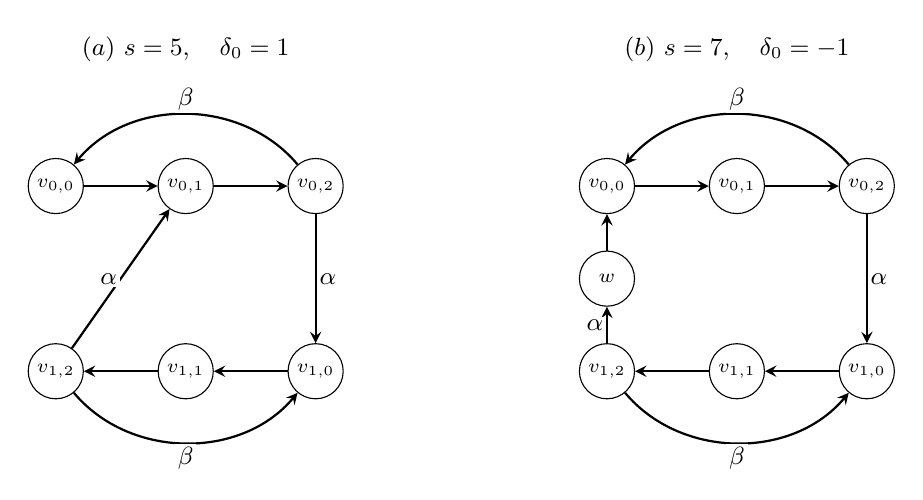
\begin{tikzpicture}[x=1.65cm,y=1.12cm,
  every node/.style={font=\small},
  vertex/.style={circle,draw,fill=white,inner sep=1.2pt,minimum size=7mm,
                 font=\scriptsize},
  edge/.style={->,>=stealth,thick},
  weight/.style={font=\small,fill=white,inner sep=1pt}]
\begin{scope}
  \node at (1,1.55) {$(a)\ s=5,\quad\delta_0=1$};
  \node[vertex] (a00) at (0,0) {$v_{0,0}$};
  \node[vertex] (a01) at (1,0) {$v_{0,1}$};
  \node[vertex] (a02) at (2,0) {$v_{0,2}$};
  \node[vertex] (a10) at (2,-2.1) {$v_{1,0}$};
  \node[vertex] (a11) at (1,-2.1) {$v_{1,1}$};
  \node[vertex] (a12) at (0,-2.1) {$v_{1,2}$};
  \draw[edge] (a00) -- (a01);
  \draw[edge] (a01) -- (a02);
  \draw[edge] (a10) -- (a11);
  \draw[edge] (a11) -- (a12);
  \draw[edge] (a02) to[out=130,in=50]
      node[weight,above] {$\beta$} (a00);
  \draw[edge] (a12) to[out=-50,in=-130]
      node[weight,below] {$\beta$} (a10);
  \draw[edge] (a02) -- node[weight,right] {$\alpha$} (a10);
  \draw[edge] (a12) -- node[weight,left] {$\alpha$} (a01);
\end{scope}
\begin{scope}[xshift=7.0cm]
  \node at (1,1.55) {$(b)\ s=7,\quad\delta_0=-1$};
  \node[vertex] (b00) at (0,0) {$v_{0,0}$};
  \node[vertex] (b01) at (1,0) {$v_{0,1}$};
  \node[vertex] (b02) at (2,0) {$v_{0,2}$};
  \node[vertex] (b10) at (2,-2.1) {$v_{1,0}$};
  \node[vertex] (b11) at (1,-2.1) {$v_{1,1}$};
  \node[vertex] (b12) at (0,-2.1) {$v_{1,2}$};
  \node[vertex] (bw) at (0,-1.05) {$w$};
  \draw[edge] (b00) -- (b01);
  \draw[edge] (b01) -- (b02);
  \draw[edge] (b10) -- (b11);
  \draw[edge] (b11) -- (b12);
  \draw[edge] (b02) to[out=130,in=50]
      node[weight,above] {$\beta$} (b00);
  \draw[edge] (b12) to[out=-50,in=-130]
      node[weight,below] {$\beta$} (b10);
  \draw[edge] (b02) -- node[weight,right] {$\alpha$} (b10);
  \draw[edge] (b12) -- node[weight,left] {$\alpha$} (bw);
  \draw[edge] (bw) -- (b00);
\end{scope}
\end{tikzpicture}
\caption{Two cyclic-transfer realizations with $m=2$ and $q=3$.
Unlabelled arrows have weight one and $\alpha+\beta=1$.
In $(a)$ the connection into block zero skips $v_{0,0}$, giving a
connection cycle of length five on six vertices. In $(b)$ the added
vertex $w$ gives a connection cycle of length seven on seven vertices.
Both graphs retain the two three-cycles closed by the return edges.}
\label{fig:realizing-graphs}
\end{figure}

If $m=1$ and $s=q$, the two terminal edges coincide and have total
weight one. The matrix is the deterministic $q$-cycle, with polynomial
$t^q-1=t^q-\beta_0-\alpha_0$, as asserted. In all other cases the
two terminal destinations are distinct.

Every simple directed cycle contains a terminal. If it chooses a return
there, the deterministic block path takes it back to the same terminal,
so it is precisely that block's $q$-cycle. If it chooses no return, it
follows the connections through every block and forms the single
$s$-cycle. Thus the complete list consists of the $m$ disjoint block
cycles, of weights $\beta_j$, and the connection cycle, of weight
$\prod_j\alpha_j$. The latter meets every block cycle at its terminal.
This description includes $q=1$, when block cycles are loops, and
$m=1,s<q$, when the connection closes a shorter cycle within its block.

In the Leibniz expansion of $\det(tI-A)$, a collection of $k$
vertex-disjoint directed cycles covering $v$ vertices contributes its
weight times $(-1)^k t^{n_0-v}$. Indeed, a cycle of length $d$ has
permutation sign $(-1)^{d-1}$ and contributes $d$ negative entries.
At a fixed point, expanding $t-a_{ii}$ selects either an unused vertex
or a loop, so the same rule applies to cycles of length one.
The collections of block cycles therefore contribute
\[
 \sum_{J\subseteq\{0,\ldots,m-1\}}
 (-1)^{|J|}t^{n_0-q|J|}\prod_{j\in J}\beta_j
 =t^{n_0-mq}\prod_{j=0}^{m-1}(t^q-\beta_j).
\]
The connection cycle can occur only alone and contributes
$-t^{n_0-s}\prod_j\alpha_j$. Their sum is
\eqref{eq:independent-characteristic}. Zero edge weights simply make
the corresponding contributions vanish, so the argument includes every
endpoint tuple. Being a polynomial identity, it includes zero roots
and their algebraic multiplicities as well.
\end{proof}

In particular, take all $\beta_j=\beta\in(0,1)$ and
$\alpha=1-\beta$. Every nonzero root $\lambda$ of
\begin{equation}\label{eq:realizing-polynomial}
 \lambda^s(\lambda^q-\beta)^m=\alpha^m\lambda^{mq}
\end{equation}
is a zero of \eqref{eq:independent-characteristic}, hence an eigenvalue
of this same stochastic matrix of order $\max\{mq,s\}$.

For consecutive order-$n$ Farey denominators, $q+s>n\ge mq$, so the theorem
applies and its order is at most $n$.
Choose \eqref{eq:equal-parameters} and use \eqref{eq:ito-attaining};
conjugation handles the reflected coordinate and an identity block gives
order $n$.  The endpoint roots are realized by $q$- and $s$-cycles.
Consequently $K_n(\theta)e^{i\theta}\in\Theta_n$ on every ray for $n\ge4$.


Combining Theorem~\ref{thm:product} with Theorems~\ref{thm:convex-product} and \ref{thm:sparse-realization} already identifies every radial maximum at its first order of occurrence $N\ge4$ with $K_N$.
At such a maximum, the unequal parameters supplied by the geometric reduction must all agree.
The remaining issue is to compare different orders without assuming the desired boundary theorem.

\section{Farey refinement and completion}
We need only two comparison operations: increase the factor count, or insert a mediant.
The first is an immediate consequence of strict convexity.

\begin{lemma}[Adding a factor]\label{lem:add-factor}
Fix $p/q<y<r/s$, $rq-ps=1$, $q<s$.
For an integer $m\ge1$, suppose
$A=2\pi(qy-p)>0$, $B_m=2\pi(r-sy)/m>0$, and $A+B_m<\pi$.
The scalar root for count $m+1$ is strictly larger than the one for count $m$.
\end{lemma}
\begin{proof}
For the old root, \eqref{eq:factor-resolution} gives an equal-parameter product with all $m$ arguments equal to $A+B_m$.
Append $\beta_{m+1}=0$, whose factor is $\omega^q$ and whose argument is $A$.
The product remains valid after changing the exterior exponent from $s-mq$ to $s-(m+1)q$, and its real phase becomes
\[
 [s-(m+1)q]2\pi y+m(A+B_m)+A=2\pi[r-(m+1)p].
\]
The enlarged tuple is unequal, since the old parameter lies in $(0,1)$.
Theorem~\ref{thm:convex-product}, now with $m+1$ factors, gives strict scalar inequality at the old root.
The new scalar left side is strictly increasing, so its root is larger.
\end{proof}

The mediant comparison will reduce to the sign of a polynomial divided
difference. The following elementary segment identity supplies that sign.
Its imaginary part has a geometric meaning: for complex vectors $v,w$,
$\operatorname{Im}(\bar v w)$ is their planar determinant, so its sign
locates $w$ relative to the oriented line in direction $v$.

\begin{lemma}[A segment comparison]
\label{thm:sector-difference}
Let $f$ be holomorphic near the segment $[a,b]\subset\mathbb C$, with $a\ne b$,
and let $\chi\in\mathbb R$.  If
$\operatorname{Im}(e^{i\chi}f'(z))>0$ on $[a,b]$, then
\[
 \operatorname{Im}\!\left(e^{i\chi}
          (\bar a-\bar b)(f(a)-f(b))\right)>0.
\]
\end{lemma}
\begin{proof}
Parametrize the segment by $z(t)=b+t(a-b)$, $0\le t\le1$.
Apply the ordinary one-variable fundamental theorem of calculus to the
real and imaginary parts of $f(z(t))$; its derivative is
$(a-b)f'(z(t))$. Multiplication by $\bar a-\bar b$ gives
\begin{equation}\label{eq:sector-difference}
 (\bar a-\bar b)(f(a)-f(b))
 =|a-b|^2\int_0^1 f'\bigl(b+t(a-b)\bigr)\,dt.
\end{equation}
Rotation by $e^{i\chi}$ and taking imaginary parts proves the claim.
\end{proof}
Only the polynomial $f(z)=z^m$ is used below. In that case the integrand
is simply $m(b+t(a-b))^{m-1}$, and the identity requires no integration
beyond the fundamental theorem of calculus for this polynomial in $t$.


\begin{corollary}[Strict mediant refinement]\label{lem:positive-mediant}
Suppose $a/b<c/d$ are consecutive in $F_{n-1}\cap[0,1/2]$ and
$b+d=n\ge4$.  On either new open interval formed by $(a+c)/n$, the new scalar
root is strictly larger than the old one.
\end{corollary}
\begin{proof}
Reflection permits $b<d$.  Put
\[
 m=\lfloor(n-1)/b\rfloor,\qquad
 A=2\pi(bx-a),\qquad B=2\pi(c-dx)/m.
\]
The old scalar root $\rho\in(0,1)$ satisfies
\begin{equation}\label{eq:old-mediant-scalar}
 \rho^{d/m}\sin A+\rho^b\sin B=\sin(A+B),
 \qquad A,B>0,\quad A+B<\pi.
\end{equation}
The mediant splits the interval according to the sign of
\[
 mB-A=2\pi\bigl((a+c)-(b+d)x\bigr).
\]
In the left child $A<mB$, keep count $m$ initially; the smaller denominator
remains $b$, and its two angles are $A,B-A/m$.
In the right child $A>mB$, reflection puts the smaller denominator $d$
first.  Its denominators are $d,b+d$, its count is one because $b<d$,
and its angles are $mB,A-mB$.  The angle sums are respectively
$A+B-A/m<\pi$ and $A<\pi$, so both scalar equations have unique roots.
Their deficits at the old radius are
\begin{align*}
 D_L&=\sin(A+B-A/m)-\rho^{(b+d)/m}\sin A
                            -\rho^b\sin(B-A/m),\\
 D_R&=\sin A-\rho^{b+d}\sin(mB)-\rho^d\sin(A-mB).
\end{align*}
Proving these deficits positive is enough: each new scalar left side
increases strictly with the radius. To find their signs, we use the old
equation to express each deficit using powers of a single radial variable. The left
child combines exponents in units of $1/m$, whereas the right child
has count one; this dictates the substitutions
\[
 \eta=A/m,\qquad u=\rho^{b/m},\qquad v=\rho^{d/m}.
\]
Set $G_m(a,b)=(\bar a-\bar b)(a^m-b^m)$.
Then the old scalar equation reads
$v\sin A+u^m\sin B=\sin(A+B)$.
In $D_L$, the mixed power is $\rho^{(b+d)/m}=uv$.
Multiplying the old equation by $u$ replaces $uv\sin A$ by
$u\sin(A+B)-u^{m+1}\sin B$. This eliminates $v$ and gives
\[
 D_L=\sin\bigl(B+(m-1)\eta\bigr)-u\sin(B+m\eta)
       -u^m\sin(B-\eta)+u^{m+1}\sin B.
\]
These four terms are the imaginary part of
$e^{iB}(e^{-i\eta}-u)(e^{im\eta}-u^m)$.
For $D_R$, both radial terms contain $v^m$, since
$\rho^{b+d}=u^mv^m$ and $\rho^d=v^m$. We therefore eliminate $u^m$
instead, using
$u^m\sin B=\sin(A+B)-v\sin A$.
After multiplication by the positive quantity $\sin B/\sin A$, the identity
\[
 \sin(A+B)\sin(mB)+\sin B\sin(A-mB)
       =\sin A\sin\bigl((m+1)B\bigr)
\]
then gives
\[
 \frac{\sin B}{\sin A}D_R
   =\sin B-v^m\sin\bigl((m+1)B\bigr)+v^{m+1}\sin(mB).
\]
This is the imaginary part of
$e^{iB}(1-ve^{-iB})(1-v^me^{imB})$; the remaining term $-v$ is real.
Thus the two deficits are instances of the same divided difference:
\begin{equation}\label{eq:mediant-differences}
 \begin{split}
 D_L&=\operatorname{Im}\!\left(e^{iB}G_m(e^{i\eta},u)\right),\\
 D_R&=\frac{\sin A}{\sin B}\,
       \operatorname{Im}\!\left(e^{iB}G_m(1,ve^{iB})\right).
 \end{split}
\end{equation}
The factors $\bar a-\bar b$ in these expressions record the directions
of the two segments. Lemma~\ref{thm:sector-difference} tests their signs
by averaging the derivatives of $f(z)=z^m$, rotated through $B$.
The left segment joins the positive real number $u$ to $e^{i\eta}$;
the right joins $1$ to $ve^{iB}$.  Their arguments lie respectively in
$[0,\eta]$ and $[0,B]$.  Since $\eta,B<\pi$, each segment lies in an open
half-plane through the origin and avoids zero.
For the left segment, the rotated derivative $e^{iB}mz^{m-1}$ has arguments in
\[
 [B,B+(m-1)\eta]\subset(0,\pi),
 \qquad B+(m-1)\eta<A+B<\pi.
\]
For the right segment its arguments lie in $[B,mB]\subset(0,\pi)$,
because the right-child condition is $mB<A<\pi$.
These statements also cover $m=1$, when the derivative is constant.
The lemma makes both imaginary parts positive; the factor $\sin A/\sin B$
is positive as well.  Each child's scalar left side is therefore below its
target at $\rho$, so its strictly increasing dependence on radius places
the child root above $\rho$.

The right child's count is already correct.  On the left, the actual count
is $\lfloor(b+d)/b\rfloor$, whereas the comparison used
$m=\lfloor(b+d-1)/b\rfloor$.
They differ precisely when $b\mid d$; coprimality of the two denominators
makes this equivalent to $b=1$.
In that case $m=d$ and the actual count is $d+1$.
Lemma~\ref{lem:add-factor} increases the radius once more, starting with
the valid angle sum $A+B-A/m<\pi$.
\end{proof}


\begin{theorem}[Monotonicity in the order]\label{thm:order-monotonicity}
For $n\ge5$ and $0\le\theta\le\pi$,
\[
 K_{n-1}(\theta)\le K_n(\theta).
\]
At inherited Farey rays there is equality.
At other rays equality holds precisely when both the containing Farey interval and its factor count remain unchanged.
\end{theorem}
\begin{proof}
Between consecutive fractions $a/b<c/d$ of $F_{n-1}$, either nothing is inserted in $F_n$, or the sole inserted fraction is $(a+c)/(b+d)$ with $b+d=n$.
Indeed, if $h/n$ is inserted, the unimodular coordinates
\[
 (n,h)=(cn-dh)(b,a)+(bh-an)(d,c)
\]
have positive integer coefficients; since $b+d\ge n$, both coefficients must be one.
On an unchanged interval the factor count stays fixed or increases by one, so the scalar equation is unchanged or Lemma~\ref{lem:add-factor} applies.
A divided interval is covered by Corollary~\ref{lem:positive-mediant}.
An inherited endpoint has value one at both orders; a new endpoint had old radius below one and has new radius one.
\end{proof}

\subsection{Small orders and the boundary}
\begin{proposition}\label{prop:low-orders}
One has $\Theta_1=\{1\}$, $\Theta_2=[-1,1]$, and, with $\xi=e^{2\pi i/3}$,
\begin{equation}\label{eq:order-three}
 \Theta_3=\operatorname{conv}\{1,\xi,\bar\xi\}\ \cup\ [-1,-1/2].
\end{equation}
On $0<\theta<\pi$, its radial maximum $R_3(\theta)$ is the order-three scalar root.
Moreover $R_3(\theta)\le K_4(\theta)$ for every $0\le\theta\le\pi$.
\end{proposition}
\begin{proof}
An order-two stochastic matrix has eigenvalues $1$ and $a-b$, where $a,b\in[0,1]$; this proves the first two claims.
If $x+iy$ is a nonreal eigenvalue of an order-three stochastic matrix, its spectrum is $1,x+iy,x-iy$.
Nonnegative diagonal entries and off-diagonal products give
\[
 1+2x=\operatorname{tr}A\ge0,\qquad
 (1+2x)^2\le3\sum_i a_{ii}^2\le3\operatorname{tr}A^2
       =3(1+2x^2-2y^2).
\]
Thus $x\ge-1/2$ and $3y^2\le(1-x)^2$, which, with $x\le1$, places the eigenvalue in the displayed triangle.
Conversely every point $a+b\xi+c\bar\xi$ of the triangle is an eigenvalue of
$aI+bC_3+cC_3^2$, where $C_3$ is a three-cycle permutation matrix,
$a,b,c\ge0$, and $a+b+c=1$.
The additional real interval is realized already at order two.

For the interval $(0,1/3)$, $q=1$ and $s=m=3$; \eqref{eq:ito-attaining} gives the segment $\omega=\beta+\alpha\xi$.
For $(1/3,1/2)$, reflected denominator ordering gives $q=2,s=3,m=1$, and the reduced equation factors as
\[
 \omega^3-\beta\omega-\alpha
   =(\omega-1)(\omega^2+\omega+\alpha)=0.
\]
Its nonreal roots have real part $-1/2$ and trace the vertical side.
These are the scalar roots by \eqref{eq:factor-resolution} and uniqueness.
In particular $\lim_{\theta\uparrow\pi}R_3(\theta)=1/2$, although $R_3(\pi)=1$.
To compare orders three and four, insert $1/4$ into $(0,1/3)$ and apply Corollary~\ref{lem:positive-mediant}; on $(1/3,1/2)$ the interval stays fixed and the count increases from one to two, so Lemma~\ref{lem:add-factor} applies.
The angle sums are strictly below $\pi$ on these open intervals by \eqref{eq:angle-budget}.
Endpoints, including the exceptional negative real ray, have the claimed comparison directly.
\end{proof}

The unit-circle classification is also elementary.
Cycles realize every root of unity of order at most $n$.
Conversely, if $Ax=\lambda x$ with $|\lambda|=1$, choose $M=\max_j|x_j|>0$ and $S=\{j:|x_j|=M\}$.
Equality in the triangle inequality shows, for every $i\in S$, that each positive transition $i\to j$ stays in $S$ and satisfies $x_j=\lambda x_i$.
There is a directed cycle in $S$ of length $\ell\le n$, and following it gives $\lambda^\ell=1$.
Thus the unit-circle points are exactly those asserted in the boundary theorem.

\begin{proof}[Completion of Theorem~\ref{thm:karpelevic}]
Fix $n\ge4$ and a ray $0\le\theta\le\pi$, and let $R_n(\theta)$ be its actual radial maximum.
Attainment gives $K_n(\theta)\le R_n(\theta)$.
On a Farey ray both sides equal one by the unit-circle classification.
Otherwise put $z=R_n(\theta)e^{i\theta}$ and let $k\le n$ be its least order of occurrence.
Then $z\ne0$, $z$ is nonreal, $|z|<1$, and $k\ge3$.
If $k=3$, Proposition~\ref{prop:low-orders} and order monotonicity give
\[
 |z|\le R_3(\theta)\le K_4(\theta)\le K_n(\theta)\le |z|.
\]
If $k\ge4$, the invariant-polygon criterion says that its multiplier first admits a polygon at $k$ vertices.
An outward enlargement admitting at most $k$ vertices would contradict its radial maximality in $\Theta_n$.
Thus Theorem~\ref{thm:product} applies.
The convex comparison and attainment give $|z|=K_k(\theta)$; then
\[
 |z|=K_k(\theta)\le K_n(\theta)\le |z|.
\]
Hence $R_n=K_n$ on every ray.
Star-shapedness gives
\[
 \Theta_n=\{re^{i\theta}:0\le r\le K_n(\theta)\},
\]
with $K_n$ extended by conjugation.
Since this radial function is positive and continuous, its graph is exactly the boundary.
Equations \eqref{eq:ito-attaining} and \eqref{eq:factor-resolution} identify its arcs with the stated Ito equations, and the endpoint limits join the prescribed roots of unity.
Proposition~\ref{prop:low-orders} supplies the remaining orders and the terminal order-three segment.
\end{proof}

% END focused-analytic.tex

% BEGIN restored-gauges-asymptotics.tex
\section{Optimal polygonal gauges}
\label{sec:gauges}

Invariant polyhedra and their Minkowski functionals are standard tools
in stability and control \cite{Bitsoris,FarinaBenvenuti,Blanchini}.
Hennet and Lasserre give the invariance condition for a rotation-dilation
on a centered regular polygon \cite[Lemma~2]{HennetLasserre}; regular
polygons also appear in constructions of polyhedral Lyapunov functions
for planar complex modes \cite{RossiColaneriShorten}. Kousoulidis and
Forni study polyhedral Lyapunov functions with prescribed complexity
\cite{KousoulidisForni}. Here the completed boundary theorem determines
the exact best contraction factor among all polygons with a prescribed
vertex bound, allowing nonregular and nonsymmetric polygons.

Let $R_\theta$ be
planar rotation and $T_{\rho,\theta}=\rho R_\theta$, with $\rho>0$.
For $N\ge4$, define
\[
 \Gamma_N(T_{\rho,\theta})=
 \inf\{\gamma>0:T_{\rho,\theta}P\subseteq\gamma P,
 \quad0\in\operatorname{int}P,
 \quad P\text{ has at most }N\text{ vertices}\},
\]
where $P$ ranges over full-dimensional polygons.  No symmetry is imposed.
Its Minkowski functional
\[
 V_P(x)=\inf\{a>0:x\in aP\}
\]
is therefore a gauge, and need not be a norm.  By
Theorem~\ref{thm:karpelevic}, the exact radial function of $\Theta_N$ is
\[
 K_N(\theta)=\max\{r:re^{i\theta}\in\Theta_N\}.
\]

\Needspace{20\baselineskip}
\begin{theorem}[Exact gauge complexity]\label{thm:gauges}
For $N\ge4$, $\rho>0$, and $0\le\theta\le\pi$,
\begin{equation}\label{eq:gauge-optimum}
 \Gamma_N(T_{\rho,\theta})=\frac{\rho}{K_N(\theta)}.
\end{equation}
The infimum is attained.  An attaining polygon satisfies
\[
 V_P(T_{\rho,\theta}x)\le
 \Gamma_N(T_{\rho,\theta})V_P(x)\qquad(x\in\R^2).
\]
Moreover,
\begin{equation}\label{eq:uniform-gauge}
 \min_{0\le\theta\le\pi}K_N(\theta)=\cos(\pi/N),\qquad
 \max_{0\le\theta\le\pi}
       \frac{\Gamma_N(T_{\rho,\theta})}{\rho}=\sec(\pi/N),
\end{equation}
and the first Farey arc has the explicit radius
\begin{equation}\label{eq:first-arc}
 K_N(\theta)=\frac{\cos(\pi/N)}{\cos(\theta-\pi/N)}
 \qquad(0\le\theta\le2\pi/N).
\end{equation}
In particular the minimum in \eqref{eq:uniform-gauge} is attained at
$\theta=\pi/N$.
\end{theorem}
\begin{proof}
For every admissible polygon and every $\gamma>0$,
\[
 \rho R_\theta P\subseteq\gamma P
 \quad\Longleftrightarrow\quad
 (\rho/\gamma)R_\theta P\subseteq P.
\]
The invariant-polygon criterion \eqref{eq:polygon-criterion} puts
$(\rho/\gamma)e^{i\theta}$ in $\Theta_N$, so
$\rho/\gamma\le K_N(\theta)$.  This proves the lower bound in
\eqref{eq:gauge-optimum}.

Conversely, the boundary multiplier $K_N(\theta)e^{i\theta}$ belongs
to $\Theta_N$.  If it is nonreal and has modulus less than one, the
criterion supplies a polygon with at most $N$ vertices; the observation
following \eqref{eq:polygon-criterion} makes it full dimensional with
zero in its interior.  At a nonreal unit-circle point, use the convex
hull of its root-of-unity orbit, whose order is at most $N$.  On the two
real rays, where $K_N=1$, use a centered square.  In each case
$K_N(\theta)R_\theta P\subseteq P$.  Rescaling this inclusion gives
attainment and the reverse bound.  Applying it to $x\in aP$ and taking
the infimum over $a$ gives the stated gauge inequality.

To find the worst angle, let $Q_N$ be the convex hull of the $N$th
roots of unity.  For $z\in Q_N$, multiplication of a convex expression
for $z$ by any vertex of $Q_N$ again gives a convex combination of the
same roots.  Thus $zQ_N\subseteq Q_N$, and the polygon criterion gives
$Q_N\subseteq\Theta_N$.  Since the inradius of $Q_N$ is $\cos(\pi/N)$,
\[
 K_N(\theta)\ge\cos(\pi/N)\qquad(0\le\theta\le\pi).
\]
For the first Farey interval, from $0/1$ to $1/N$, the scalar equation
\eqref{eq:radial} has $q=1$, $s=m=N$, $A=\theta$, and
$B=2\pi/N-\theta$.  It is linear in its radial variable, and gives
\[
 K_N(\theta)=
 \frac{\sin(2\pi/N)}{\sin\theta+\sin(2\pi/N-\theta)}
 =\frac{\cos(\pi/N)}{\cos(\theta-\pi/N)}.
\]
Evaluation at $\theta=\pi/N$ proves the minimum; the gauge formula
then proves the maximum.
\end{proof}

In the plane a polygon has as many sides as vertices.  Thus $N$ also
bounds the number of linear pieces in the representation of $V_P$ as a
maximum of linear functionals.  A strictly contracting gauge with this
bound exists exactly when
\[
 \rho<K_N(\theta).
\]
If the polygon may be chosen after the angle is known, but the same
vertex bound must work for every angle, the exact condition is
$\rho<\cos(\pi/N)$.  The restriction $N\ge4$ matters on the negative
real ray: although $-1\in\Theta_3$, an inclusion $-P\subseteq P$ implies
$P=-P$, and a full-dimensional triangle cannot be centrally symmetric.

\section{Farey asymptotics and vertex complexity}
\label{sec:asymptotic}

The preceding radius and contraction formulas are exact at every order.
We now approximate their values as $N$ increases.  These estimates are
consequences of the completed boundary theorem; they introduce no error
into its description of $\Theta_N$.

The arithmetic viewpoint has a separate history. \DJ okovi\'c used
cyclic polygons generated by powers of a complex number in his
simplification of the stochastic eigenvalue region \cite{Djokovic}.
Dubuc and Malik developed the connection among these convex hulls,
trinomial equations, and Farey sequences \cite{DubucMalik}; Dubuc and
Zaoui subsequently studied the fractal dimension of unions of trinomial
arcs \cite{DubucZaoui}. In particular, for a trinomial Farey arc
associated with $p/q<r/s$ and $s>q>2$, Dubuc and Malik prove the
one-sided estimate $|z|^s\ge1-\pi^2/(qs)$
\cite[Theorem~13.1]{DubucMalik}.
The prescribed-ray scalar characterization of Kirkland, Laffey, and
\v{S}migoc \cite{KirklandLaffeySmigoc} gives a later point of comparison.
Here the matrix order varies: the scalar equation yields a relative
asymptotic that records both Farey denominators and the position within
the interval. It refines the one-sided estimate in the trinomial
subcase and also applies when the factor count is larger.

For an angle strictly between two order-$N$ Farey rays, orient the
interval as before so that its smaller endpoint denominator comes first:
\[
 \frac pq<y<\frac rs,\qquad q<s,\qquad rq-ps=1,
 \qquad m=\lfloor N/q\rfloor.
\]
Here $y=\theta/(2\pi)$ or $1-\theta/(2\pi)$ according to the reflection.
Its relative coordinate is
\[
 t=s(qy-p)\in(0,1),\qquad
 y-\frac pq=\frac{t}{qs},\qquad
 \frac rs-y=\frac{1-t}{qs}.
\]
The coordinate $t$ is allowed to approach either endpoint as rapidly as
the Farey data permit.

\begin{theorem}[Uniform radial deficit]\label{thm:farey-asymptotic}
Uniformly over all open Farey intervals of order $N$ and all $0<t<1$,
\begin{equation}\label{eq:uniform-farey-asymptotic}
 1-K_N(\theta)=
 \frac{2\pi^2t(1-t)}{qs}
 \left(\frac{t}{s}+\frac{1-t}{mq}\right)
 \bigl(1+O(N^{-2})\bigr)
 \qquad(N\to\infty).
\end{equation}
The implied constant is absolute.  Thus, for a fixed irrational
$x\in(0,1/2)$, let $p_N/q_N<y_N<r_N/s_N$ be its successive oriented
Farey intervals, with $y_N=x$ or $1-x$, and set
$m_N=\lfloor N/q_N\rfloor$, $t_N=s_N(q_Ny_N-p_N)$.  Then
\[
 1-K_N(2\pi x)\sim
 \frac{2\pi^2t_N(1-t_N)}{q_Ns_N}
 \left(\frac{t_N}{s_N}+\frac{1-t_N}{m_Nq_N}\right),
\]
without a lower bound on $t_N$ or $1-t_N$.
\end{theorem}
\begin{proof}
Farey adjacency gives $q+s>N$.  It follows that $s>N/2$; also
$mq>N/2$, because $N<(m+1)q$ and $m\ge1$.  Set
\[
 A=\frac{2\pi t}{s},\qquad
 B=\frac{2\pi(1-t)}{mq},\qquad
 H(u)=u^{s/m}\sin A+u^q\sin B.
\]
Both angles and their sum are $O(N^{-1})$, uniformly in the interval
and in $t$.  With $K=K_N(\theta)$, the exact scalar equation is
$H(K)=\sin(A+B)$.  Its defect at radius one factors as
\begin{equation}\label{eq:sine-defect}
 \begin{split}
 D:=H(1)-\sin(A+B)
 &=4\sin(A/2)\sin(B/2)\sin((A+B)/2)\\
 &=\frac{AB(A+B)}2\bigl(1+O(N^{-2})\bigr).
 \end{split}
\end{equation}
The last estimate is relative, even near an endpoint.  Dividing each
sine by its own positive argument gives three factors of the form
$1+O(N^{-2})$; no division by $t$ or $1-t$ is used in the error bound.
Similarly,
\begin{equation}\label{eq:farey-derivative}
 \begin{split}
 H'(1)&=\frac{s}{m}\sin A+q\sin B\\
 &=\frac{2\pi}{m}
   \left(t\frac{\sin A}{A}+(1-t)\frac{\sin B}{B}\right)
 =\frac{2\pi}{m}\bigl(1+O(N^{-2})\bigr).
 \end{split}
\end{equation}
Here the two weights sum to one, so this estimate also stays uniform
as either weight tends to zero.

The mean-value theorem gives
\[
 D=(1-K)H'(\xi)\qquad(K<\xi<1).
\]
It remains to replace $H'(\xi)$ by $H'(1)$ accurately enough.  We do
this in two steps.  First, the regular-polygon bound in
Theorem~\ref{thm:gauges} gives $1-K=O(N^{-2})$, hence
$|\log\xi|=O(N^{-2})$.  Since both exponents $q,s/m$ are at most
$N$, each power $\xi^{q-1}$ and $\xi^{s/m-1}$ differs from one by
$O(N^{-1})$.  The two derivative terms are positive, so
\[
 \frac{H'(\xi)}{H'(1)}=1+O(N^{-1}).
\]
Together with $D=O(N^{-3})$ and \eqref{eq:farey-derivative}, this
improves the initial deficit estimate to
\[
 1-K=O(mN^{-3})=O\bigl((qN^2)^{-1}\bigr).
\]
For the second step use the sharper exponent bound
$s/m\le N/m<2q$.  Now $|\log\xi|=O((qN^2)^{-1})$, so both powers
in the derivative differ from one by $O(N^{-2})$.  Positivity again gives
\[
 \frac{H'(\xi)}{H'(1)}=1+O(N^{-2}).
\]
Combining the mean-value identity with
\eqref{eq:sine-defect}--\eqref{eq:farey-derivative} yields
\[
 1-K=\frac{mAB(A+B)}{4\pi}\bigl(1+O(N^{-2})\bigr).
\]
Substitution of the two angles proves
\eqref{eq:uniform-farey-asymptotic}.  All constants used above are
independent of the interval and of $t$, which also proves the stated
fixed-irrational asymptotic.
\end{proof}

Thus the displayed leading term approximates the positive deficit
$1-K_N$, with relative error bounded by a constant times $N^{-2}$.
At a Farey endpoint the deficit and leading term are both exactly zero;
the relative assertion concerns the open interval.  For a general
irrational angle, the denominators and the position inside its current
interval both matter.  Badly approximable angles give a simpler rate.
Recall that $x$ is badly approximable if some $c_x>0$ satisfies
\[
 \left|x-\frac ab\right|\ge\frac{c_x}{b^2}
 \qquad\text{for every rational }a/b.
\]
We write $a_N\asymp_x b_N$ when their ratio is bounded above and below
by positive constants depending only on $x$.

\begin{corollary}[Contraction loss and vertex budgets]
\label{cor:complexity-asymptotic}
Let $x\in[0,1/2]$ and $N\ge4$.  If $x=a/b$ is rational in lowest
terms, $K_N(2\pi x)=1$ exactly when $b\le N$.  For irrational $x$, the radius
is strictly below one at every finite order.  For badly approximable $x$,
\begin{equation}\label{eq:badly-approximable-loss}
 1-K_N(2\pi x)\asymp_x N^{-3},\qquad
 \frac{\Gamma_N(T_{\rho,2\pi x})}{\rho}-1\asymp_x N^{-3}.
\end{equation}
Uniformly in angle,
\begin{equation}\label{eq:uniform-relative-loss}
 \max_{0\le\theta\le\pi}
 \left(\frac{\Gamma_N(T_{\rho,\theta})}{\rho}-1\right)
 =\sec(\pi/N)-1\sim\frac{\pi^2}{2N^2}.
\end{equation}
For $\varepsilon>0$, define
\[
 B_x(\varepsilon)=\min\left\{N\ge4:
   \frac{\Gamma_N(T_{\rho,2\pi x})}{\rho}-1\le\varepsilon\right\}.
\]
Then $B_x(\varepsilon)\asymp_x\varepsilon^{-1/3}$ for badly
approximable $x$ as $\varepsilon\downarrow0$.  If the same accuracy
must hold for every angle, the required budget is exactly
\begin{equation}\label{eq:uniform-vertex-budget}
 B_{\mathrm{unif}}(\varepsilon)
 =\max\left\{4,
   \left\lceil\frac{\pi}{\arccos((1+\varepsilon)^{-1})}\right\rceil\right\}
 \sim\frac{\pi}{\sqrt{2\varepsilon}}.
\end{equation}
These relative-loss budgets do not depend on $\rho>0$.
\end{corollary}
\begin{proof}
The rational and irrational statements follow from the unit-circle
classification in Theorem~\ref{thm:karpelevic}.  Bad approximability
is preserved by replacing $x$ with $1-x$.  For the oriented Farey
interval its two endpoint inequalities give
\[
 t\ge c_xs/q,\qquad 1-t\ge c_xq/s.
\]
Since $q<s$ and $t<1$, the first inequality yields
$c_xs<q<s$.  Thus the denominators are comparable.  It also gives
$t\ge c_x$, and the second inequality now gives $1-t>c_x^2$.
Together with $q+s>N$ and $s\le N$, this proves
\[
 q\asymp_x s\asymp_x N,\qquad mq\asymp N.
\]
Every factor in the leading term of
\eqref{eq:uniform-farey-asymptotic} therefore has the stated scale:
the denominator $qs$ is of order $N^2$, while the parenthesis is of
order $N^{-1}$.  This proves the first estimate in
\eqref{eq:badly-approximable-loss}.  The second follows from
\[
 \frac{\Gamma_N(T_{\rho,2\pi x})}{\rho}-1
 =\frac{1-K_N(2\pi x)}{K_N(2\pi x)}
\]
and $K_N\to1$.

Equation~\eqref{eq:uniform-gauge} gives the exact maximum in
\eqref{eq:uniform-relative-loss}; the Taylor expansion of the secant
gives its asymptotic.  The finite-order losses at an irrational angle
are positive, so $B_x(\varepsilon)\to\infty$ as
$\varepsilon\downarrow0$.  Inverting the two-sided $N^{-3}$ bound
then gives upper and lower constant multiples of $\varepsilon^{-1/3}$.
Finally, solving $\sec(\pi/N)-1\le\varepsilon$ for the integer
$N\ge4$ gives \eqref{eq:uniform-vertex-budget}, and the expansion
$\arccos((1+\varepsilon)^{-1})\sim\sqrt{2\varepsilon}$ gives its
last term.
\end{proof}

% END restored-gauges-asymptotics.tex

% BEGIN restored-comparisons.tex
\clearpage
\appendix
\section{Quantitative and unequal-exponent comparisons}
\label{app:comparisons}

The convex comparison contains more information than the sharp radius.
Keeping its Jensen gap measures how far an admissible factor tuple is from
equal coefficients. Allowing different exponents leads to a related
optimization, in which the available argument range of each factor becomes
an upper constraint.

\subsection{Quantitative rigidity on the prescribed phase}

\begin{proposition}[Quantitative rigidity]\label{prop:quantitative-rigidity}
Under the hypotheses of Theorem~\ref{thm:convex-product}, put
\[
 F(u)=\log\sin M-\log\sin(M-u),\qquad
 \bar u=A+B,\qquad J=\sum_{j=1}^mF(u_j)-mF(\bar u),
\]
and let
\[
 D_\rho=\sin(A+B)-\rho^{s/m}\sin A-\rho^q\sin B.
\]
Then
\begin{equation}\label{eq:jensen-gap}
 J\ge\frac12\sum_{j=1}^m(u_j-\bar u)^2,
 \qquad
 D_\rho=\rho^{s/m}\sin A\bigl(e^{J/m}-1\bigr).
\end{equation}
In particular,
\begin{equation}\label{eq:argument-variance-bound}
 \sum_{j=1}^m(u_j-\bar u)^2
 \le2m\log\left(1+\frac{D_\rho}{\rho^{s/m}\sin A}\right)
 \le\frac{2mD_\rho}{\rho^{s/m}\sin A}.
\end{equation}
With $\bar\beta=m^{-1}\sum_j\beta_j$ and
$c_\rho=\rho^q\sin A/(1+\rho^q)^2$, one also has
\begin{equation}\label{eq:coefficient-variance-bound}
 \sum_{j=1}^m(\beta_j-\bar\beta)^2
 \le c_\rho^{-2}\sum_{j=1}^m(u_j-\bar u)^2.
\end{equation}
For fixed interior Farey data and angles, both variances are
$O(\rho_\ast-\rho)$ as an admissible family approaches the scalar root
$\rho_\ast$. The constants are uniform on compact subsets of an open Farey
interval when $\rho$ is bounded away from zero.
\end{proposition}
\begin{proof}
Since $(1-\Re\omega^q)/\Im\omega^q=-\cot M$, the normalized-line
function from Theorem~\ref{thm:convex-product} is
\[
 \mathcal D(u)=\cos u-\cot M\sin u
 =\frac{\sin(M-u)}{\sin M}=e^{-F(u)}.
\]
The prescribed real phase gives $\sum_j u_j=m\bar u$.
The curvature bound \eqref{eq:one-factor-convexity} gives $F''\ge1$,
so Taylor's inequality at $\bar u$ gives
\[
 F(u_j)\ge F(\bar u)+F'(\bar u)(u_j-\bar u)
                         +\tfrac12(u_j-\bar u)^2.
\]
The linear terms cancel on summation, proving the gap bound.
For its relation to the radius, the modulus identity gives
$J/m=(q-s/m)\log\rho+\log\mathcal D(A+B)$, so
\[
 e^{J/m}
 =\rho^{q-s/m}\mathcal D(A+B)
 =\frac{\sin(A+B)-\rho^q\sin B}{\rho^{s/m}\sin A},
\]
where the last equality is the normalized-line evaluation used there.
Rearranging proves the exact identity in \eqref{eq:jensen-gap}; taking
logarithms and using $\log(1+x)\le x$ proves
\eqref{eq:argument-variance-bound}.

To pass from arguments to coefficients, \eqref{eq:one-factor-convexity} yields
\[
 \frac{du}{d\beta}
 =\frac{\rho^q\sin A}{|\rho^qe^{iA}-\beta|^2}
 \ge\frac{\rho^q\sin A}{(1+\rho^q)^2}=c_\rho>0.
\]
Thus $|\beta_i-\beta_j|\le c_\rho^{-1}|u_i-u_j|$.
Apply this to the pairwise variance identity
\[
 \sum_{j=1}^m(x_j-\bar x)^2
       =\frac1m\sum_{i<j}(x_i-x_j)^2
\]
to obtain \eqref{eq:coefficient-variance-bound}.
Finally, for $H(t)=t^{s/m}\sin A+t^q\sin B$,
\[
 D_\rho=H(\rho_\ast)-H(\rho)
       =H'(\rho_\ast)(\rho_\ast-\rho)+o(\rho_\ast-\rho).
\]
The stated order and compact uniformity follow from the positive denominators
in the variance bounds and continuity of the displayed quantities.
\end{proof}
Here admissibility includes both the finite product and its specified real
phase lift. The conclusion controls this factor tuple; it makes no
matrix-distance assertion for arbitrary eigenvalues near the boundary.

\subsection{Different exponents and constrained angular allocation}

With different exponents the normalized factors lie on different lines.
Measuring each argument from its limiting direction $M_j$ gives an angular
deficit $v_j=M_j-u_j$. The available deficits $U_j$ need not agree.
The optimal choice shares the deficit equally among the remaining factors
after each binding upper constraint is met.

\begin{theorem}[Unequal-exponent product bound]\label{thm:unequal-product-bound}
Let $m\ge1$, let $q_1,\ldots,q_m$ be positive integers, let $e\in\mathbb Z$,
and write $z=\rho e^{i\theta}$ with $\rho>0$. Suppose
$A_j=\operatorname{Arg}(z^{q_j})\in(0,\pi)$ and $0\le\beta_j<1$.
Put
\[
 M_j=\operatorname{Arg}(z^{q_j}-1),\qquad
 u_j=\operatorname{Arg}(z^{q_j}-\beta_j),\qquad
 U_j=M_j-A_j,\quad v_j=M_j-u_j,
\]
and assume the product and its specified real phase
\begin{equation}\label{eq:unequal-product-phase}
 z^e\prod_{j=1}^m(z^{q_j}-\beta_j)=\prod_{j=1}^m(1-\beta_j),
 \qquad e\theta+\sum_{j=1}^m u_j=2\pi L,\quad L\in\mathbb Z.
\end{equation}
Then $0<v_j\le U_j<\pi$ and
\[
 S:=\sum_{j=1}^mM_j+e\theta-2\pi L=\sum_{j=1}^m v_j,
 \qquad 0<S\le\sum_{j=1}^mU_j.
\]
If $S<\sum_jU_j$, let $c\in(0,\max_jU_j)$ be the unique solution of
$\sum_j\min(c,U_j)=S$; at equality set $c=\max_jU_j$.
The vector
\[
 v_j^*=\min(c,U_j)
\]
is the unique maximizer of $\prod_j\sin v_j$ subject to
$0<v_j\le U_j$ and $\sum_jv_j=S$. Consequently
\begin{equation}\label{eq:unequal-sharp-product}
 \rho^e\prod_{j=1}^m\sin M_j
   =\prod_{j=1}^m\sin v_j
   \le\prod_{j=1}^m\sin v_j^*,
\end{equation}
with equality precisely when $v_j=v_j^*$ for every $j$. More precisely,
\begin{equation}\label{eq:unequal-quadratic-deficit}
 \log\frac{\prod_j\sin v_j^*}{\rho^e\prod_j\sin M_j}
       \ge\frac12\sum_{j=1}^m(v_j-v_j^*)^2.
\end{equation}
If $S/m\le\min_jU_j$, this reduces to
\[
 \rho^e\prod_{j=1}^m\sin M_j\le\sin^m(S/m),
\]
with equality exactly when $v_1=\cdots=v_m=S/m$.
\end{theorem}
\begin{proof}
As $\beta$ increases from zero towards one,
$\operatorname{Arg}(z^{q_j}-\beta)$ increases from $A_j$ towards $M_j$.
Thus $0<v_j\le U_j<\pi$. Put $w_j=z^{q_j}$ and
$c_j=(1-\Re w_j)/\Im w_j=-\cot M_j$; here $c_j$ may have either sign.
The normalized-line identity
$\Re g_j+c_j\Im g_j=1$, with $g_j=(w_j-\beta_j)/(1-\beta_j)$,
gives
\[
 \frac{|w_j-\beta_j|}{1-\beta_j}
       =\frac1{\cos u_j+c_j\sin u_j}
       =\frac{\sin M_j}{\sin v_j}.
\]
Taking moduli in \eqref{eq:unequal-product-phase} proves the equality in
\eqref{eq:unequal-sharp-product}; the phase gives $S=\sum_jv_j$.
The function $c\mapsto\sum_j\min(c,U_j)$ is continuous and strictly increasing
until it reaches $\sum_jU_j$. This proves the existence and uniqueness of
the stated $c$, and makes $v^*$ feasible.

Set $\Phi(v)=\sum_j\log\sin v_j$. Its Hessian is diagonal with entries
$-\csc^2v_j\le-1$, so every feasible vector satisfies
\[
 \Phi(v)-\Phi(v^*)
 \le\sum_j\cot(v_j^*)(v_j-v_j^*)
                          -\tfrac12\sum_j(v_j-v_j^*)^2.
\]
When $S<\sum_jU_j$, the equal coordinate sums cancel the common slope
$\cot c$. The remaining linear term is
\[
 \sum_{U_j<c}(\cot U_j-\cot c)(v_j-U_j)\le0.
\]
Each coefficient is positive because cotangent decreases on $(0,\pi)$,
and each difference is nonpositive by its upper constraint.
It follows that $v^*$ uniquely maximizes $\Phi$, with precisely the stated
quadratic deficit. Exponentiation gives the sharp product bound and its
equality case. At total saturation the feasible set is the singleton $v=U$.
If $S/m\le\min_jU_j$, the choice $c=S/m$ gives the final assertion.
\end{proof}

For the equal-exponent data of Theorem~\ref{thm:convex-product}, all $M_j=M$
and $U_j=M-A$, while
$S=m(M-A-B)<m(M-A)$. No upper constraint binds, and equality gives
$v_j=M-A-B$, hence $u_j=A+B$ and equal coefficients.
With unequal exponents it is the angular deficits that agree where the
constraints do not bind. The theorem is a product comparison on a prescribed
phase; identifying a spectral boundary would still require a realization
and an independent argument that its selected branch is outermost.

% END restored-comparisons.tex

% BEGIN restored-matrix-family.tex
\section{Independent-parameter realizations}\label{app:matrix-family}
Theorem~\ref{thm:sparse-realization} gives the full characteristic
polynomial of the graph in Figure~\ref{fig:realizing-graphs}.
We now record its support and connectivity, its endpoint matrices,
and the equality case on a prescribed Farey arc.

\begin{proposition}[Structure of the realization family]\label{prop:family-structure}
Let $A(\boldsymbol\beta)$ be the matrix constructed in
Theorem~\ref{thm:sparse-realization}, and suppose $q<s$.
If every $\beta_j\in(0,1)$, it is irreducible and has exactly $n_0+m$
positive entries: $m$ rows have two, and every other row has one.
If also $\gcd(q,s)=1$, it is primitive.
For every parameter tuple in $[0,1]^m$ and every $n\ge n_0$,
$A(\boldsymbol\beta)\oplus I_{n-n_0}$ is stochastic of order $n$
and retains all its eigenvalues.
\end{proposition}
\begin{proof}
Suppose all return and connection weights are positive. The connections reach every block, and the returns then reach every vertex of each block; inserted vertices also lie on a connection. The graph is therefore strongly connected. Any terminal lies on its block cycle of length $q$ and on the connection cycle of length $s$.
If $\gcd(q,s)=1$, every integer $L\ge(q-1)s$ has the form $aq+bs$ with $a,b\ge0$: choose $b\in\{0,\ldots,q-1\}$ so that $bs\equiv L\pmod q$. Given any two vertices, take a path from the first to a fixed terminal and a path from there to the second. Inserting the two terminal cycles supplies every sufficiently large additional length. There are finitely many vertex pairs, so every sufficiently high power of the matrix is entrywise positive. This proves primitivity directly.

The two destinations of each terminal row are distinct. For $m\ge2$ they lie in different blocks or one is an inserted vertex; for $m=1$, the assumption $q<s$ requires an inserted connection. Hence there are exactly $m$ rows with two positive entries and $n_0-m$ with one. The identity-block extension has characteristic polynomial $(t-1)^{n-n_0}\det(tI-A)$.
\end{proof}

For consecutive order-$n$ Farey denominators $q<s$, take $m=\lfloor n/q\rfloor$. Then $q+s>n\ge mq$ verifies the realization hypothesis, $n_0\le n$, and Farey coprimality gives primitivity for interior weights. When every parameter equals $\beta$, writing $\alpha=1-\beta$ reduces the characteristic polynomial to
\[
 \begin{cases}
 (t^q-\beta)^m-\alpha^m t^{mq-s},&s\le mq,\\
 t^{s-mq}(t^q-\beta)^m-\alpha^m,&s>mq.
 \end{cases}
\]
At the two constant endpoint tuples this becomes, respectively,
\[
 \det(tI-A(\mathbf1))=t^{n_0-mq}(t^q-1)^m,
 \qquad
 \det(tI-A(\mathbf0))=t^{n_0-s}(t^s-1).
\]
Thus the endpoint roots of unity are realized in the same continuous matrix family. Formula~\eqref{eq:independent-characteristic} also remains valid at every mixed tuple of zero, unit, and interior weights; irreducibility is asserted only for interior tuples.

The equality statement for the scalar bound singles out one tuple within this larger family. It uses the prescribed real phase: the characteristic equation by itself records the phase only modulo $2\pi$.

\begin{corollary}[Equality within the realization family]\label{cor:family-equality}
Let $n\ge4$, and let $p/q<r/s$, $q<s$, be the denominator-oriented form of two consecutive fractions in $F_n^+$. Put $m=\lfloor n/q\rfloor$ and suppose $0\le\beta_j<1$.
Let $\omega=\rho e^{i\vartheta}$, $0<\rho<1$, be a root of \eqref{eq:independent-characteristic}, with
\[
 \frac pq<\frac{\vartheta}{2\pi}<\frac rs,
 \qquad A=q\vartheta-2\pi p,\qquad B=\frac{2\pi r-s\vartheta}{m}.
\]
Set $M=\operatorname{Arg}(\omega^q-1)$ and $u_j=\operatorname{Arg}(\omega^q-\beta_j)\in[A,M)$. If
\[
 (s-mq)\vartheta+\sum_{j=0}^{m-1}u_j=2\pi(r-mp),
\]
then, with $\theta=\min\{\vartheta,2\pi-\vartheta\}$,
\[
 \rho\le K_n(\theta).
\]
Equality holds if and only if all parameters agree. At equality their common value is uniquely
\[
 \beta_*=\frac{K_n(\theta)^q\sin B}{\sin(A+B)}.
\]
\end{corollary}
\begin{proof}
Since $\omega\ne0$, its characteristic equation is equivalent to
\[
 \omega^{s-mq}\prod_j(\omega^q-\beta_j)=\prod_j(1-\beta_j).
\]
The Farey angle calculation \eqref{eq:angle-budget} gives $A,B>0$ and $A+B<\pi$. Together with the assumed real phase, this is exactly the input to Theorem~\ref{thm:convex-product}. It gives the bound and equality precisely when the parameters agree. In that case their factor arguments all equal $A+B$; taking real and imaginary parts as in \eqref{eq:factor-resolution} gives the stated common value. Conversely, \eqref{eq:equal-parameters} supplies that tuple and realizes the scalar radius.
\end{proof}

Along the selected open arc, $\beta_*$ tends to one at the denominator-$q$ endpoint and to zero at the denominator-$s$ endpoint. Indeed, $K_n\to1$ there, while respectively $A\to0$ and $B\to0$ in its formula. The other angle stays strictly between zero and $\pi$ by \eqref{eq:angle-budget}. The matrices realizing the arc therefore converge to the two endpoint matrices displayed above.

% END restored-matrix-family.tex

% BEGIN focused-declarations.tex
\section*{Author information}
\noindent\textsuperscript{1}Department of Business Technology and Operations,
Data Analytics Laboratory, Vrije Universiteit Brussel (VUB),
Pleinlaan 2, 1050 Brussels, Belgium.\par
\noindent\textsuperscript{2}imec-SMIT, Vrije Universiteit Brussel,
Pleinlaan 9, 1050 Brussels, Belgium.\par
\noindent\textsuperscript{3}School of Engineering and Applied Sciences,
Harvard University, Cambridge, Massachusetts 02138, USA.\par
\noindent\href{mailto:brecht.verbeken@vub.be}{brecht.verbeken@vub.be};
\href{mailto:vincent.ginis@vub.be}{vincent.ginis@vub.be}.

\section*{Funding}
Vincent Ginis acknowledges support from the Research Foundation--Flanders
(FWO) under grants G032822N and G0K9322N.

\section*{Use of generative artificial intelligence}
The source manuscript was developed with OpenAI's ChatGPT and Codex
and Anthropic's Claude as research companions and editorial tools.
These systems were used to explore proof strategies, alternative
approaches, and connections between ideas, and to clarify, reorganize,
and refine the exposition. OpenAI's Codex was also used in preparing
this structural revision, including its mathematical exploration,
exposition, diagrams, and computational checks.

% END focused-declarations.tex

% BEGIN focused-references.tex
\begin{thebibliography}{99}
\raggedright
\bibitem{VG} B. Verbeken and V. Ginis,
\emph{A Geometric Proof of the Karpelevi\v{c} Theorem}, supplied manuscript,
PDF dated 27 August 2026, 77 pages.
\bibitem{DD} N. A. Dmitriev and E. B. Dynkin,
On characteristic roots of stochastic matrices,
\emph{Izv. Akad. Nauk SSSR Ser. Mat.} \textbf{10} (1946), 167--184;
English translation, \emph{Amer. Math. Soc. Transl. Ser. 2} \textbf{140}, 57--77.
\bibitem{Karp} F. I. Karpelevi\v{c},
On the characteristic roots of matrices with nonnegative elements,
\emph{Izv. Akad. Nauk SSSR Ser. Mat.} \textbf{15} (1951), 361--383;
English translation, \emph{Amer. Math. Soc. Transl. Ser. 2} \textbf{140}, 79--100.
\bibitem{Ito} H. Ito,
A new statement about the theorem determining the region of eigenvalues of stochastic matrices,
\emph{Linear Algebra Appl.} \textbf{267} (1997), 241--246.
\href{https://doi.org/10.1016/S0024-3795(97)80052-3}{doi:10.1016/S0024-3795(97)80052-3}.
\bibitem{JP} C. R. Johnson and P. Paparella,
A matricial view of the Karpelevi\v{c} theorem,
\emph{Linear Algebra Appl.} \textbf{520} (2017), 1--15.
\href{https://arxiv.org/abs/1611.06970}{arXiv:1611.06970}.
\bibitem{MNP} D. N. Munger, A. L. Nickerson and P. Paparella,
Demystifying the Karpelevi\v{c} theorem,
\emph{Linear Algebra Appl.} \textbf{702} (2024), 46--62.
\href{https://arxiv.org/abs/2309.03849}{arXiv:2309.03849}.
\bibitem{Brauer} A. Brauer,
Limits for the characteristic roots of a matrix. IV. Applications to stochastic matrices,
\emph{Duke Math. J.} \textbf{19} (1952), 75--91.
\href{https://doi.org/10.1215/S0012-7094-52-01910-8}{doi:10.1215/S0012-7094-52-01910-8}.
\bibitem{Goddard} L. S. Goddard,
Note on a matrix theorem of A. Brauer and its extension,
\emph{Canad. J. Math.} \textbf{7} (1955), 527--530.
\href{https://doi.org/10.4153/CJM-1955-055-6}{doi:10.4153/CJM-1955-055-6}.

\bibitem{BermanPlemmons} A. Berman and R. J. Plemmons,
\emph{Nonnegative Matrices in the Mathematical Sciences},
Classics in Applied Mathematics \textbf{9}, SIAM, Philadelphia, PA, 1994.
Corrected republication of the 1979 edition.
\bibitem{Bitsoris} G. Bitsoris,
On the positive invariance of polyhedral sets for discrete-time systems,
\emph{Systems Control Lett.} \textbf{11}(3) (1988), 243--248.
\bibitem{Blanchini} F. Blanchini,
Set invariance in control,
\emph{Automatica} \textbf{35}(11) (1999), 1747--1767.
\bibitem{Coxeter} H. S. M. Coxeter,
\emph{Projective Geometry}, 2nd ed., Springer-Verlag, New York, 1987.
\bibitem{DubucMalik} S. Dubuc and A. Malik,
Convex hull of powers of a complex number, trinomial equations and the Farey sequence,
\emph{Numer. Algorithms} \textbf{2}(1) (1992), 1--32.
\bibitem{DubucZaoui} S. Dubuc and M. Zaoui,
The fractal dimension of a union of trinomial arcs,
\emph{Fractals} \textbf{4}(4) (1996), 555--562.
\bibitem{FarinaBenvenuti} L. Farina and L. Benvenuti,
Invariant polytopes of linear systems,
\emph{IMA J. Math. Control Inform.} \textbf{15}(3) (1998), 233--240.
\bibitem{HardyWright} G. H. Hardy and E. M. Wright,
\emph{An Introduction to the Theory of Numbers}, 6th ed.,
Oxford University Press, Oxford, 2008.
Revised by D. R. Heath-Brown and J. H. Silverman.
\bibitem{HarlevJohnsonLim} A. Harlev, C. R. Johnson and D. Lim,
The doubly stochastic single eigenvalue problem: A computational approach,
\emph{Exp. Math.} \textbf{31}(3) (2022), 936--945.
\href{https://arxiv.org/abs/1908.03647}{arXiv:1908.03647}.
\bibitem{HennetLasserre} J.-C. Hennet and J.-B. Lasserre,
Construction of positively invariant polytopes for stable linear systems,
\emph{IFAC Proc. Volumes} \textbf{26}(2, Part 2) (1993), 315--318.
\href{https://doi.org/10.1016/S1474-6670(17)48952-X}{doi:10.1016/S1474-6670(17)48952-X}.
\bibitem{KirklandLeslie} S. Kirkland,
An eigenvalue region for Leslie matrices,
\emph{SIAM J. Matrix Anal. Appl.} \textbf{13}(2) (1992), 507--529.
\href{https://doi.org/10.1137/0613033}{doi:10.1137/0613033}.
\bibitem{KirklandLaffeySmigoc} S. Kirkland, T. Laffey and H. \v{S}migoc,
The Karpelevi\v{c} region revisited,
\emph{J. Math. Anal. Appl.} \textbf{490}(2) (2020), article 124332.
\bibitem{KirklandSmigoc} S. Kirkland and H. \v{S}migoc,
Stochastic matrices realising the boundary of the Karpelevi\v{c} region,
\emph{Linear Algebra Appl.} \textbf{635} (2022), 116--138.
\bibitem{KousoulidisForni} D. Kousoulidis and F. Forni,
Polyhedral Lyapunov functions with fixed complexity,
in \emph{2021 60th IEEE Conference on Decision and Control (CDC)},
IEEE, 2021, 3293--3298.
\href{https://arxiv.org/abs/2103.03613}{arXiv:2103.03613}.
\bibitem{LevickPereiraKribs} J. Levick, R. Pereira and D. W. Kribs,
The four-dimensional Perfect--Mirsky conjecture,
\emph{Proc. Amer. Math. Soc.} \textbf{143}(5) (2015), 1951--1956.
\bibitem{Djokovic} D. \v{Z}. \DJ{}okovi\'c,
Cyclic polygons, roots of polynomials with decreasing nonnegative coefficients, and eigenvalues of stochastic matrices,
\emph{Linear Algebra Appl.} \textbf{142} (1990), 173--193.
\href{https://doi.org/10.1016/0024-3795(90)90266-F}{doi:10.1016/0024-3795(90)90266-F}.
\bibitem{PerfectMirsky} H. Perfect and L. Mirsky,
Spectral properties of doubly-stochastic matrices,
\emph{Monatsh. Math.} \textbf{69}(1) (1965), 35--57.
\bibitem{RanTeng} A. C. M. Ran and Z. E. Teng,
The nonnegative inverse eigenvalue problem with prescribed zero patterns in dimension three,
\emph{Electron. J. Linear Algebra} \textbf{40} (2024), 506--537.
\href{https://doi.org/10.13001/ela.2024.7965}{doi:10.13001/ela.2024.7965}.
\bibitem{RossiColaneriShorten} F. Rossi, P. Colaneri and R. Shorten,
Pad\'e discretization for linear systems with polyhedral Lyapunov functions,
\emph{IEEE Trans. Automat. Control} \textbf{56}(11) (2011), 2717--2722.
\bibitem{Schneider} R. Schneider,
\emph{Convex Bodies: The Brunn--Minkowski Theory}, 2nd expanded ed.,
Encyclopedia of Mathematics and its Applications \textbf{151},
Cambridge University Press, Cambridge, 2014.
\bibitem{Slater} N. B. Slater,
Gaps and steps for the sequence $n\theta\bmod1$,
\emph{Proc. Cambridge Philos. Soc.} \textbf{63}(4) (1967), 1115--1123.
\href{https://doi.org/10.1017/S0305004100042195}{doi:10.1017/S0305004100042195}.
\bibitem{Swift} J. Swift,
\emph{The Location of Characteristic Roots of Stochastic Matrices},
M.Sc. thesis, McGill University, Montreal, 1972.
\href{https://escholarship.mcgill.ca/concern/theses/12579t72d}{McGill repository}.
\bibitem{VagenendeFourCycle} B. Vagenende, B. Verbeken, A. Algaba and M.-A. Guerry,
On the spectral region of 4-cycle stochastic matrices, preprint, 2026.
\href{https://arxiv.org/abs/2605.06743}{arXiv:2605.06743}.
\bibitem{VagenendeStar} B. Vagenende, B. Verbeken and M.-A. Guerry,
Star-convexity of the eigenvalue regions for stochastic matrices and certain subclasses,
\emph{Mathematics} \textbf{13}(12) (2025), article 2038.
\href{https://doi.org/10.3390/math13122038}{doi:10.3390/math13122038}.
\bibitem{VagenendeMonotone} B. Vagenende, B. Verbeken and M.-A. Guerry,
Eigenvalue regions and realising monotone stochastic matrices,
\emph{Electron. J. Linear Algebra} \textbf{42} (2026), 387--398.
\href{https://doi.org/10.13001/ela.2026.10159}{doi:10.13001/ela.\allowbreak 2026.10159}.
\bibitem{VGNCycle} B. Verbeken and V. Ginis,
On the spectral region of $n$-cycle stochastic matrices, preprint, 2026.
\href{https://arxiv.org/abs/2606.10143}{arXiv:2606.10143}.
\bibitem{VGTypeII} B. Verbeken and V. Ginis,
Stochastic realisers of non-degenerate full-degree Type II reduced Ito polynomials,
Zenodo preprint, 28 July 2026.
\href{https://doi.org/10.5281/zenodo.21653759}{doi:10.5281/zenodo.21653759}.
\bibitem{VGTypeIII} B. Verbeken and V. Ginis,
The Type III realisation conjecture of Kirkland and \v{S}migoc,
preprint, 2026.
\href{https://arxiv.org/abs/2607.27219}{arXiv:2607.27219}.
\end{thebibliography}

% END focused-references.tex
\end{document}
